\chapter{Resultados y conclusiones}
	\label{conclusiones}

La síntesis e implementación del acelerador se llevó a cabo mediante la herramienta Vivado 2015.3, utilizando la estrategia por defecto para ambos procesos. El dispositivo xc7z045ffg900-2 se fijó como objetivo para la obtención de los resultados de ocupación y rendimiento. El código rtl del proyecto no invoca elementos exclusivos para dispositivos de Xilinx, por lo que el código puede ser portado a elementos de familias de Altera obteniendo resultados de ocupación similares para dispositivos con LUTs de 6 entradas.

La tabla \ref{table:ch7_network_core_ocu} muestra la ocupación de una red con 25 nodos de procesamiento. Elementos de memoria distribuida son utilizados para la implementación de bancos de registros y registros de segmentación.

\begin{table}[]
	\centering
		\begin{tabular}{lllll}
			Recurso & Cantidad & Utilizacion \% &  &  \\\hline
			LUT     & 25016    & 11.44          &  &  \\
			LUTRAM  & 3240     & 4.60           &  &  \\
			FF      & 21200    & 4.85           &  &  \\
			IO      & 662      & ~              &  & 
		\end{tabular}
	\caption{Ocupación para acelerador con 25 nodos de procesamiento y 10 nodos frontera de soporte}
	\label{table:ch7_network_core_ocu}
\end{table}

La estructura regular del acelerador permite estimar los recursos necesarios para escalar la red a un mayor número de nodos, la tabla \ref{table:ch7_nodo_procesamiento_ocu} muestra los recursos necesarios para la implementación de un nodo de procesamiento, sea central o terminal, de manera individual. El elemento de procesamiento está formado por una cadena feistel con un número de rondas programable. La unidad funcional fue diseñada para habilitar diversos escenarios de evaluación de rendimiento del acelerador. 

Dado su rol de elementos de soporte, los nodos frontera no representan un consumo significativo de recursos. La tabla \ref{table:ch7_nodo_frontera_ocu} muestra los recursos necesarios para la implementación de nodos frontera. Para el acelerador en evaluación, los nodos frontera representan el 3.39\% de las LUTs requeridas por la red y el 1.17\% de flip flops del sistema.

\begin{table}[]
	\centering
		\begin{tabular}{lllll}
			recurso & router & interfaz de red & procesador & nodo de red \\\hline
			LUT     & 619    & 225             & 9          & 850         \\
			FF      & 374    & 330             & 134        & 838        
		\end{tabular}
	\caption{Recursos necesarios para la implementación de nodos incorporando un elemento de procesamiento. Los resultados de ocupación se mantienen válidos para nodos terminales o nodos centrales.}
	\label{table:ch7_nodo_procesamiento_ocu}
\end{table}

\begin{table}[]
	\centering
		\begin{tabular}{lll}
			Recurso & Estimado &  \\\hline
			LUT     & 85       &  \\
			FF      & 25       &  \\
		\end{tabular}
	\caption{Recursos necesarios para lógica de soporte del acelerador.}
	\label{table:ch7_nodo_frontera_ocu}
\end{table}



\subsection{Resultados de rendimiento}
	\label{ch7_resultados_de_rendimiento}

De manera tradicional los resultados de rendimiento para redes en chip se presentan como una relación entre el tráfico ofrecido y el tráfico servido, sin embargo, la red utilizada en este trabajo tiene como aplicación destino un acelerador, por lo que es deseable mantener la red en un estado de saturación constante. La \ref{table:ch7_throughtput} presenta los resultados de rendimiento bajo diversas cargas de trabajo.


% Please add the following required packages to your document preamble:
% \usepackage[table,xcdraw]{xcolor}
% If you use beamer only pass "xcolor=table" option, i.e. \documentclass[xcolor=table]{beamer}
\begin{table}[]
\centering
\begin{tabular}{cc}
\hline
\rowcolor[HTML]{343434} 
{\color[HTML]{FFFFFF} Trafico Demandado} & {\color[HTML]{FFFFFF} Rendimiento (Gbps)} \\ \hline
10\%                                     & 15.25                                     \\
\rowcolor[HTML]{EFEFEF} 
20\%                                     & 22.71                                     \\
30\%                                     & 26.88                                     \\
\rowcolor[HTML]{EFEFEF} 
40\%                                     & 32.25                                     \\ \hline
50\%                                     & 35.92                                     \\
\rowcolor[HTML]{EFEFEF} 
60\%                                     & 35.81                                     \\
70\%                                     & 35.60                                     \\
\rowcolor[HTML]{EFEFEF} 
80\%                                     & 35.62                                     \\
90\%                                     & 35.58                                     \\
\rowcolor[HTML]{EFEFEF} 
100\%                                    & 35.30                                    
\end{tabular}
	\caption{Resultados de rendimientos del acelerador}
	\label{table:ch7_throughtput}
\end{table}


Los resultados de la tabla \ref{table:ch7_throughtput} representan el promedio del comportamiento de 10 ejecuciones de cada simulación, utilizando un generador de números pseudo-aleatorios para inicializar los inyectores de trafico a la red. Vale la pena resaltar que el que la red alcanzo su punto de saturación en la demanda de trafico del 40\%, a partir de este punto la red ya no es capaz de manejar trafico extra. Los promedios de latencia para la ejecución de cargas de trabajo sintéticas bajo diferentes escenarios de trafico demandado se presentan en la tabla \ref{table:ch7_latency}.

\begin{table}[]
	\centering
		\begin{tabular}{ll}
			Latencia promedio          & 660          \\
			Latencia máxima            & 3357         \\
			Latencia mínima            & 200         
		\end{tabular}
	\caption{Latencia de tránsito de paquetes a través de la red}
	\label{table:ch7_latency}
\end{table}



\subsection{Conclusiones}
	\label{ch7_conclusiones}

Los resultados obtenidos de la evaluación parcial de la red muestran el potencial del trabajo como se puede apreciar en la tabla \ref{ch7_comparacion_rendimiento}, sin embargo el desarrollo de un perfil de rendimiento bajo otros escenarios es indispensable para optimizar el sistema.


\begin{sidewaystable}

\centering
\begin{tabular}{@{}ccccccccc@{}}
\toprule
\rowcolor[HTML]{656565} 
{\color[HTML]{FFFFFF} \textbf{NoC}} & {\color[HTML]{FFFFFF} \textbf{Topología}}                                         & {\color[HTML]{FFFFFF} \textbf{\begin{tabular}[c]{@{}c@{}}Relacion\\ con EP\end{tabular}}} & {\color[HTML]{FFFFFF} \textbf{\begin{tabular}[c]{@{}c@{}}Algoritmo de\\ calculo de\\ ruta\end{tabular}}} & {\color[HTML]{FFFFFF} \textbf{\begin{tabular}[c]{@{}c@{}}Tipo de\\ conmutacion\end{tabular}}} & {\color[HTML]{FFFFFF} \textbf{\begin{tabular}[c]{@{}c@{}}frecuencia\\ de\\ operación\end{tabular}}} & {\color[HTML]{FFFFFF} \textbf{\begin{tabular}[c]{@{}c@{}}Ocupación\\ (Slices)\end{tabular}}} & {\color[HTML]{FFFFFF} \textbf{\begin{tabular}[c]{@{}c@{}}Ancho de\\ palabra de\\ datos (bits)\end{tabular}}} & {\color[HTML]{FFFFFF} \textbf{\begin{tabular}[c]{@{}c@{}}Ancho\\ de banda\end{tabular}}} \\ \midrule
PnoC                                & crossbar                                                                          & \begin{tabular}[c]{@{}c@{}}red\\ indirecta\end{tabular}                                   & \begin{tabular}[c]{@{}c@{}}tablas de \\ ruteo\end{tabular}                                               & \begin{tabular}[c]{@{}c@{}}conmutación\\ de circuitos\end{tabular}                            & 126 MHz                                                                                             & 1223                                                                                         & 8                                                                                                            & NP                                                                                       \\
\rowcolor[HTML]{EFEFEF} 
CuNoC                               & malla                                                                             & \begin{tabular}[c]{@{}c@{}}red\\ indirecta\end{tabular}                                   & DOR XY                                                                                                   & \begin{tabular}[c]{@{}c@{}}Store \&\\ forward\end{tabular}                                    & 241 MHz                                                                                             & 128                                                                                          & 32                                                                                                           & NP                                                                                       \\
Quark                               & spidergon                                                                         & \begin{tabular}[c]{@{}c@{}}red\\ directa\end{tabular}                                     & \begin{tabular}[c]{@{}c@{}}calculo de \\ cuadrante\end{tabular}                                          & wormhole                                                                                      & NP                                                                                                  & 1453                                                                                         & 32                                                                                                           & NP                                                                                       \\
\rowcolor[HTML]{EFEFEF} 
Hermes                              & malla                                                                             & \begin{tabular}[c]{@{}c@{}}red\\ directa\end{tabular}                                     & DOR XY                                                                                                   & wormhole                                                                                      & 25 MHz                                                                                              & 316                                                                                          & 10                                                                                                           & 500 Mbps                                                                                 \\
MoCReS                              & malla                                                                             & \begin{tabular}[c]{@{}c@{}}red\\ directa\end{tabular}                                     & DOR XY                                                                                                   & \begin{tabular}[c]{@{}c@{}}virtual\\ cut-through\end{tabular}                                 & 357 MHz                                                                                             & 282                                                                                          & 8                                                                                                            & 2.85 Gbps                                                                                \\
\rowcolor[HTML]{EFEFEF} 
SoCWire                             & múltiple                                                                          & \begin{tabular}[c]{@{}c@{}}red\\ directa\end{tabular}                                     & \begin{tabular}[c]{@{}c@{}}XY\\ modificado\end{tabular}                                                  & wormhole                                                                                      & 180 MHz                                                                                             & 1270                                                                                         & 32                                                                                                           & 2800 Mbps                                                                                \\
SoCIN                               & malla                                                                             & \begin{tabular}[c]{@{}c@{}}red\\ directa\end{tabular}                                     & DOR XY                                                                                                   & wormhole                                                                                      & 49 MHz                                                                                              & 2100                                                                                         & 32                                                                                                           & NP                                                                                       \\
\rowcolor[HTML]{EFEFEF} 
RoC                                 & anillo                                                                            & \begin{tabular}[c]{@{}c@{}}red\\ directa\end{tabular}                                     & NP                                                                                                       & NP                                                                                            & 138 MHz                                                                                             & 144                                                                                          & 32                                                                                                           & 552 Mbps                                                                                 \\
RMBoC                               & \begin{tabular}[c]{@{}c@{}}bus\\ dinámico\end{tabular}                            & \begin{tabular}[c]{@{}c@{}}red\\ indirecta\end{tabular}                                   & a medida                                                                                                 & \begin{tabular}[c]{@{}c@{}}circuit\\ switched\end{tabular}                                    & 94 MHz                                                                                              & 5084                                                                                         & 32                                                                                                           & NP                                                                                       \\
DyNoC                               & \cellcolor[HTML]{EFEFEF}\begin{tabular}[c]{@{}c@{}}malla\\ irregular\end{tabular} & \cellcolor[HTML]{EFEFEF}\begin{tabular}[c]{@{}c@{}}red\\ indirecta\end{tabular}           & \cellcolor[HTML]{EFEFEF}\begin{tabular}[c]{@{}c@{}}variante \\ DOR XY\end{tabular}                       & \cellcolor[HTML]{EFEFEF}NP                                                                    & \cellcolor[HTML]{EFEFEF}391 MHz                                                                     & \cellcolor[HTML]{EFEFEF}1689                                                                 & \cellcolor[HTML]{EFEFEF}32                                                                                   & \cellcolor[HTML]{EFEFEF}NP                                                               \\

Tesis                             & \cellcolor[HTML]{EFEFEF} \begin{tabular}[c]{@{}c@{}}malla\end{tabular}                         &\cellcolor[HTML]{EFEFEF} \begin{tabular}[c]{@{}c@{}}red\\ directa\end{tabular}                                   & \cellcolor[HTML]{EFEFEF} \begin{tabular}[c]{@{}c@{}}WFM \\ modificado\end{tabular}                                               & \cellcolor[HTML]{EFEFEF} \begin{tabular}[c]{@{}c@{}}virtual\\ cut-through\end{tabular}                                 &\cellcolor[HTML]{EFEFEF} 250 MHz                                                                                              &\cellcolor[HTML]{EFEFEF} 212                                                                                          &\cellcolor[HTML]{EFEFEF} 32                                                                                                           &\cellcolor[HTML]{EFEFEF} 35.30 Gbps                                                                                       \\ \bottomrule
\end{tabular}
\caption{Tabla comparativa de trabajos similares con el diseño propuesto en esta tesis. NP - Dato no proporcionado en referencia}
\label{ch7_comparacion_rendimiento}


\end{sidewaystable}



Permitir que la red distribuya el trabajo entre todos los elementos de procesamiento resulta una técnica efectiva de administración de elementos funcionales, sin embargo los puertos de salida de la red muestran promedios de trabajo de alrededor de 26\% del tiempo de ejecución, este resultado abre la puerta a la posibilidad de reducir el número de puertos de salida bajo una penalización sobre la saturación de canales de la red.  

La distribución equitativa de paquetes entre nodos frontera destino y puertos de salida de la red no aparenta ser el mejor patrón de tráfico para el acelerador. Las figuras \ref{fig:ch6_histogramas_1} y \ref{fig:ch6_histogramas_2} muestran los histogramas de latencia para cada puertos de salida, los resultados no uniformes de tiempos de salida de paquetes es evidencia de un desbalance en la transmisión de paquetes. El fenómeno de desbalance entre puertos de salida es resultado de la naturaleza parcialmente adaptativa del algoritmo \textit{west first minimal}, el cual presenta un mayor grado de adaptabilidad para paquetes en tránsito en dirección \textit{x-} $\longrightarrow$ \textit{x+}, mientras paquetes en dirección \textit{x+} $\longrightarrow$ \textit{x-} solo cuentan con una dirección de avance. La implementación del algoritmo de encaminamiento \textit{XY} podría ofrecer una alternativa al algoritmo utilizado durante las pruebas de rendimiento realizadas, sin embargo el mayor número de restricciones para la toma de rutas entre nodos no lo perfila como una solución viable.

Para mantener los resultados de rendimiento presentados en el capitulo \ref{ch:acelerador_multinucleo}, se requiere de una estructura de memoria capaz de alimentar de manera constante al acelerador. La capacidad de los facilitadores de datos a la red limitará su rendimiento absoluto.

\begin{figure}[ht!]
\captionsetup[subfigure]{justification=centering}
     \begin{center}
%
        \begin{subfigure}[b]{0.4\textwidth}
        	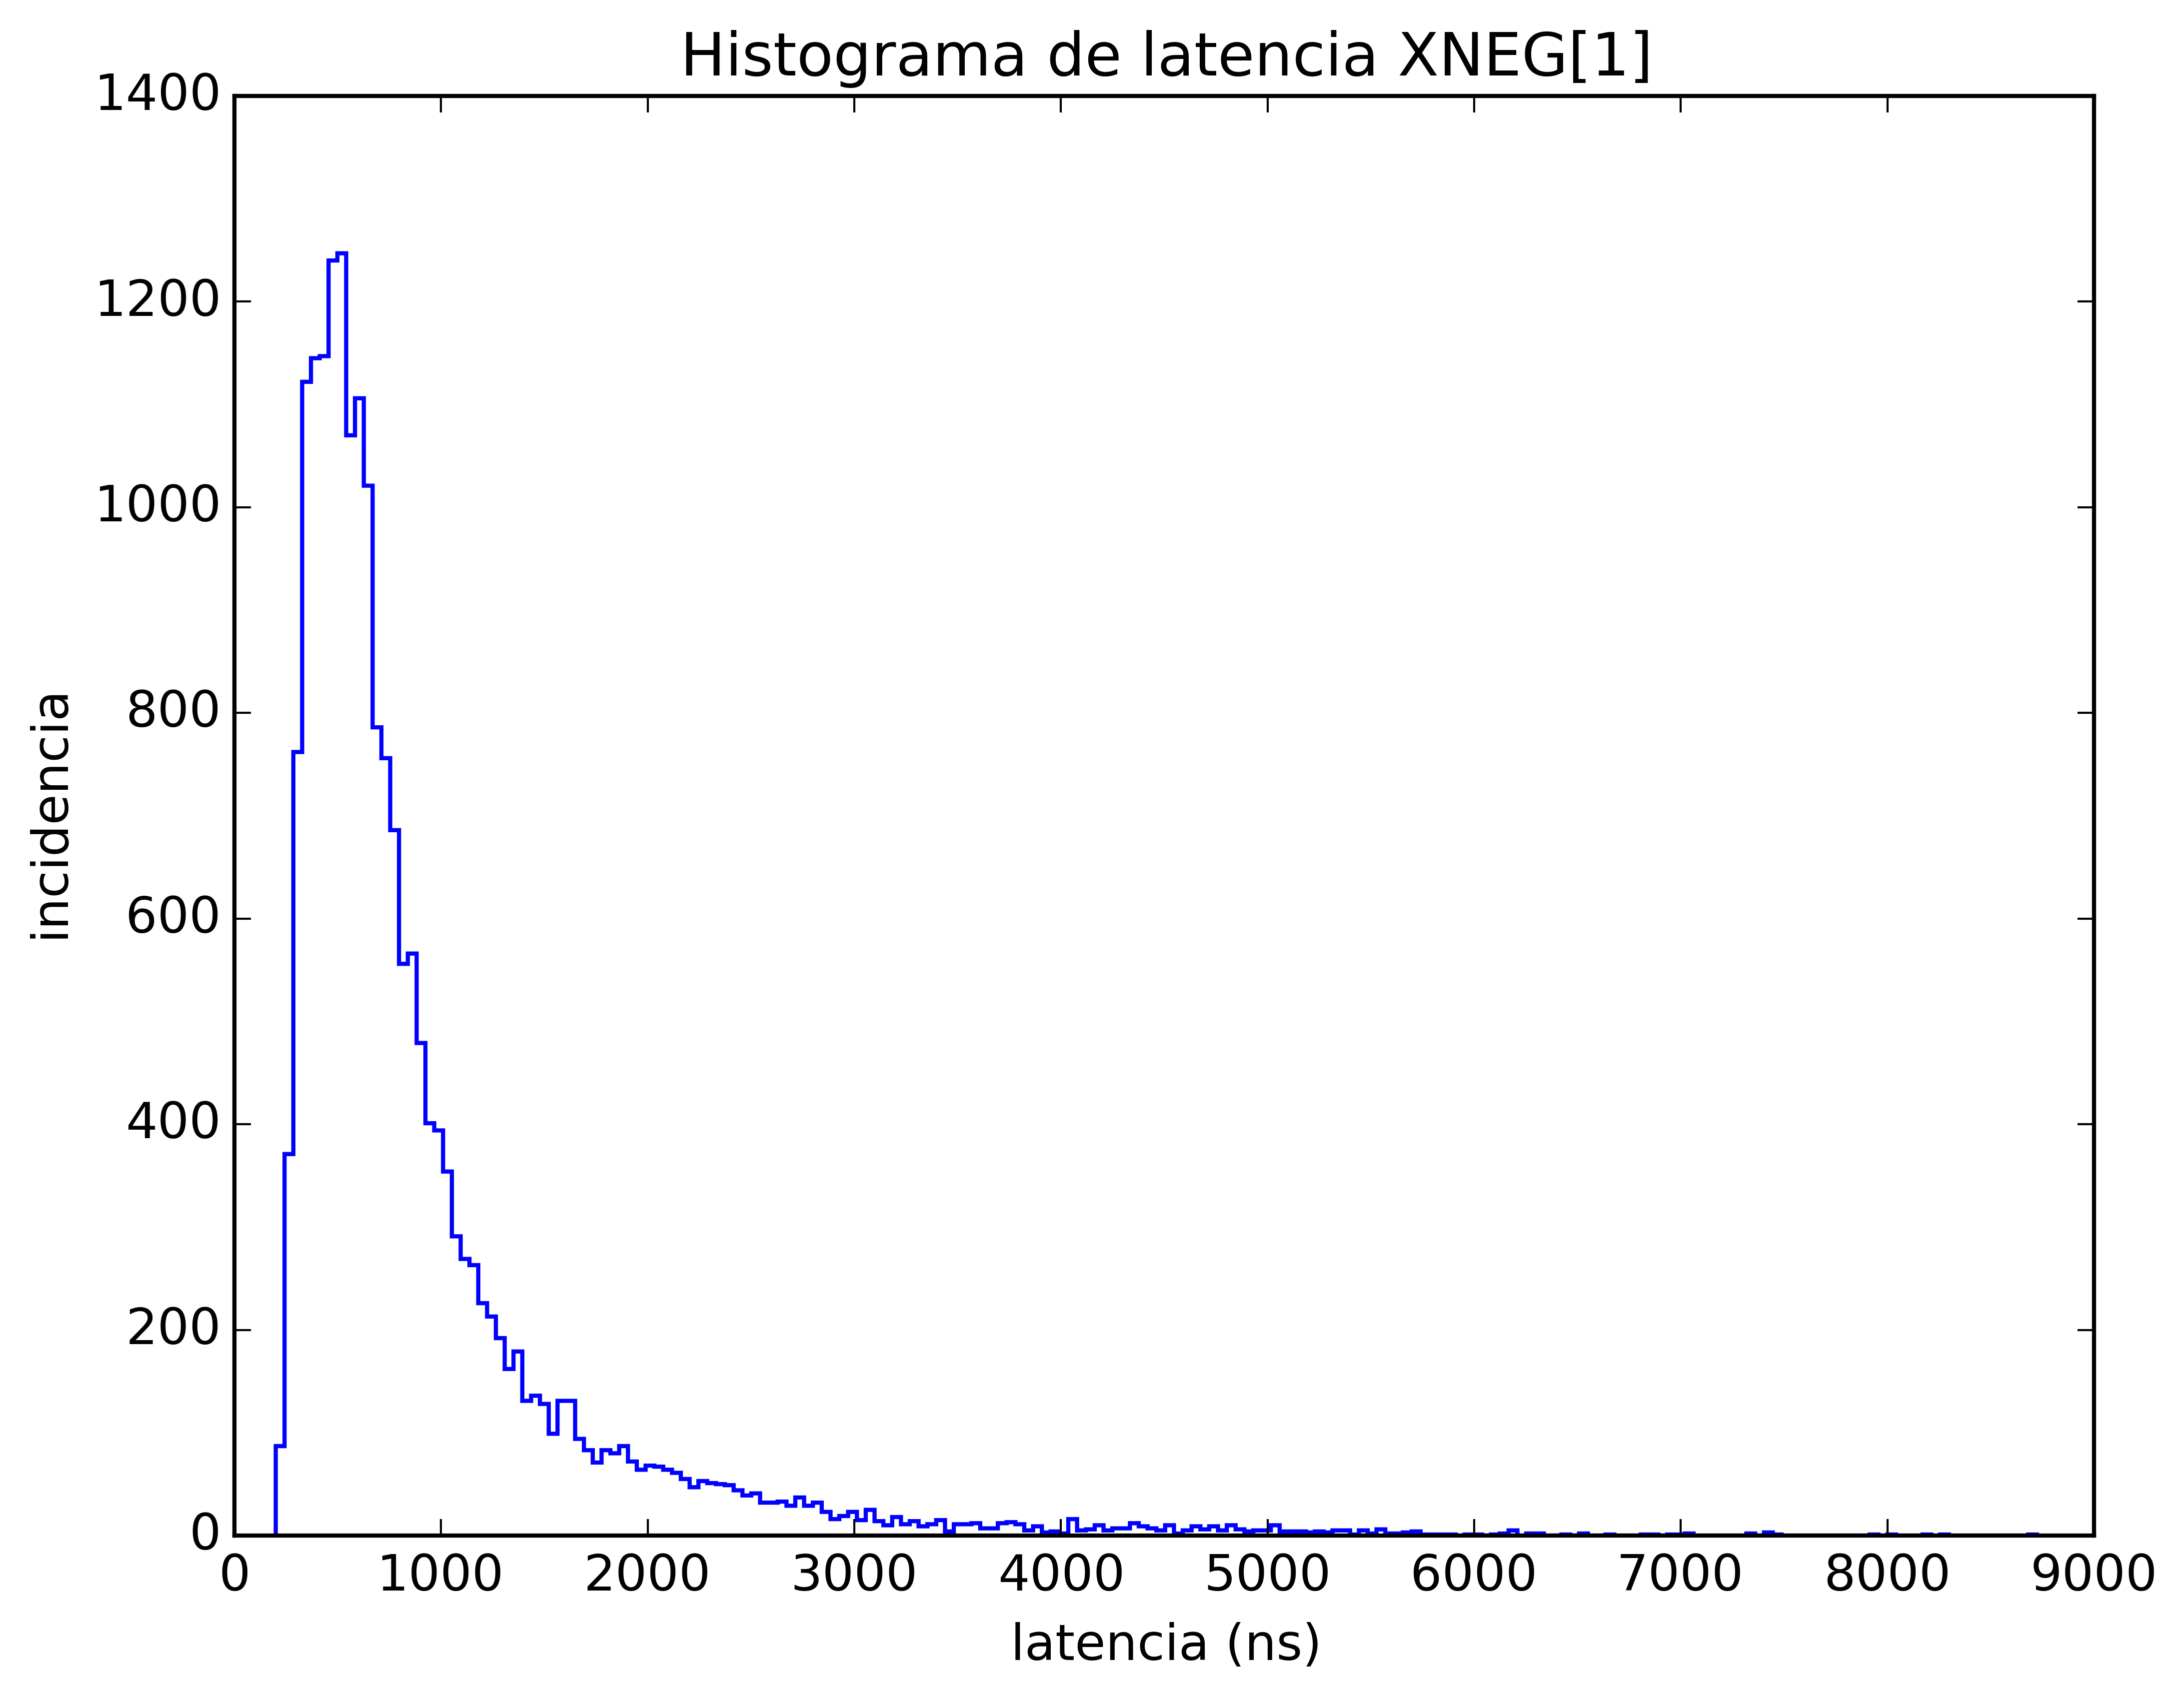
\includegraphics[width=\textwidth]{figures/ch6_histograma_source_1.png}
		    \caption{}
		    \label{fig:histograma_1}
	    \end{subfigure}
	    ~ %add desired spacing between images, e. g. ~, \quad, \qquad, \hfill etc. 
	      %(or a blank line to force the subfigure onto a new line)
	    \begin{subfigure}[b]{0.4\textwidth}
	    	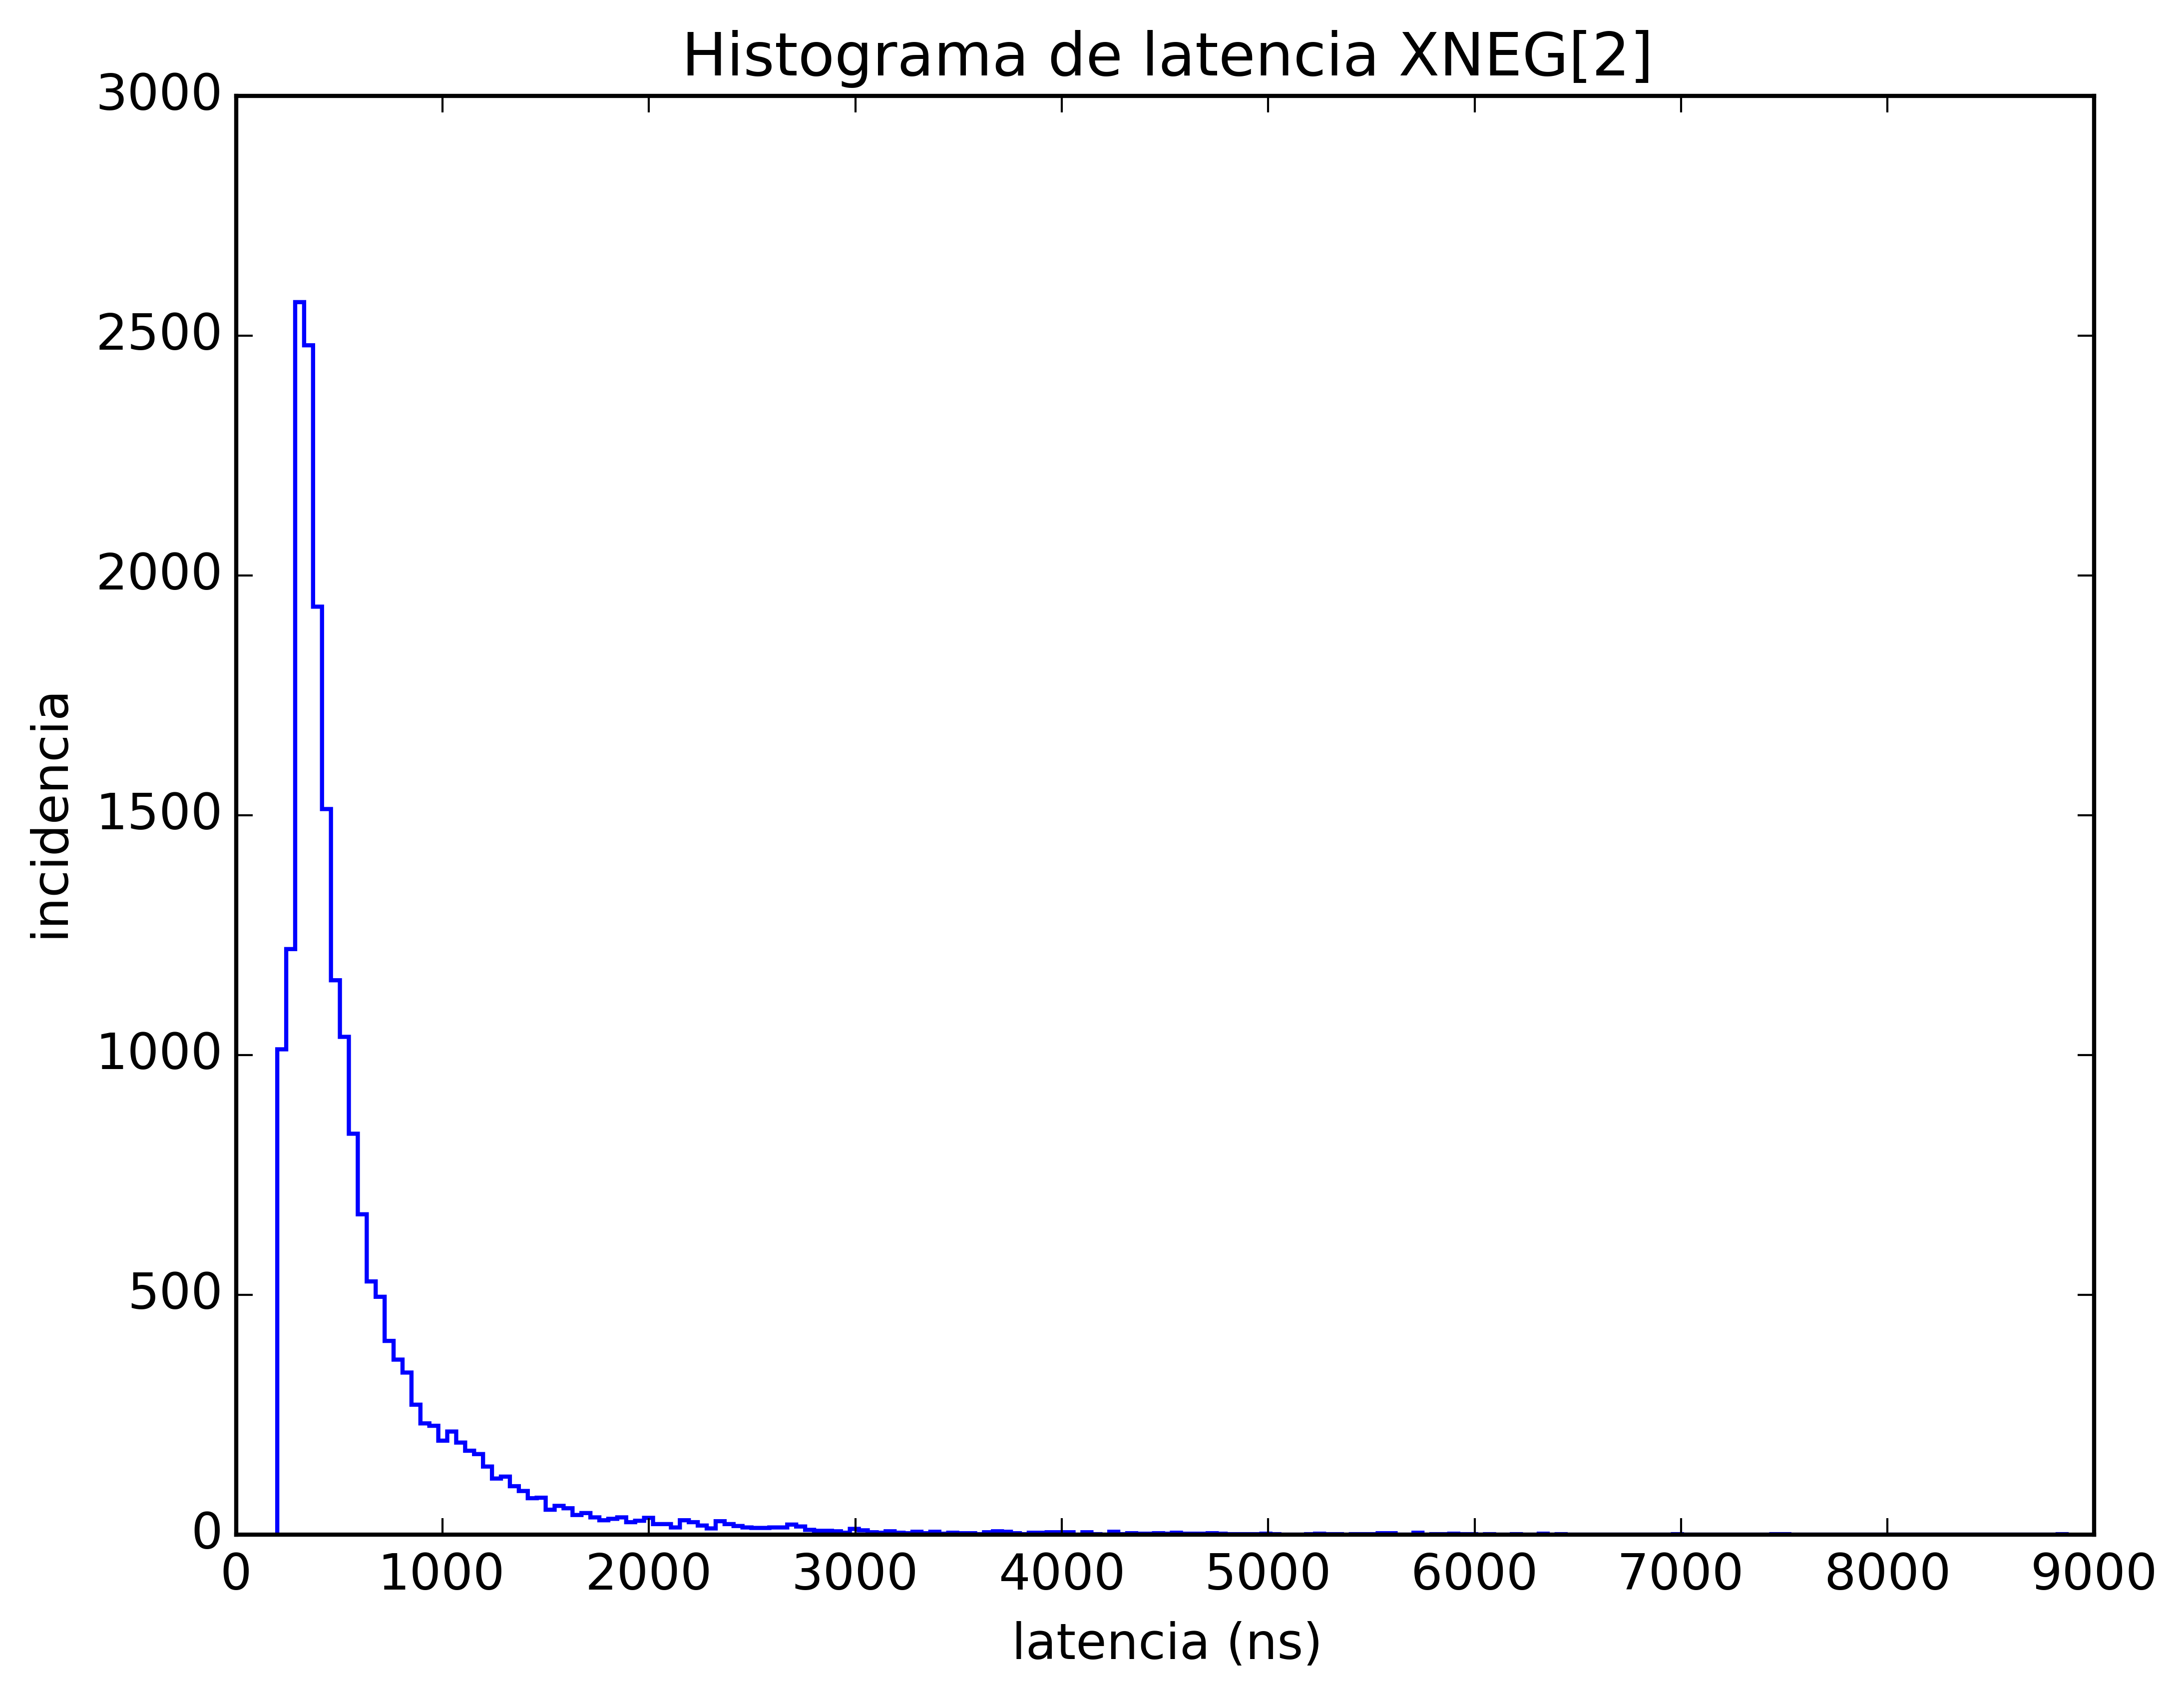
\includegraphics[width=\textwidth]{figures/ch6_histograma_source_2.png}
		    \caption{}
		    \label{fig:histograma_2}
	    \end{subfigure}
	    ~ %add desired spacing between images, e. g. ~, \quad, \qquad, \hfill etc. 
	    %(or a blank line to force the subfigure onto a new line)
	    \begin{subfigure}[b]{0.4\textwidth}
	    	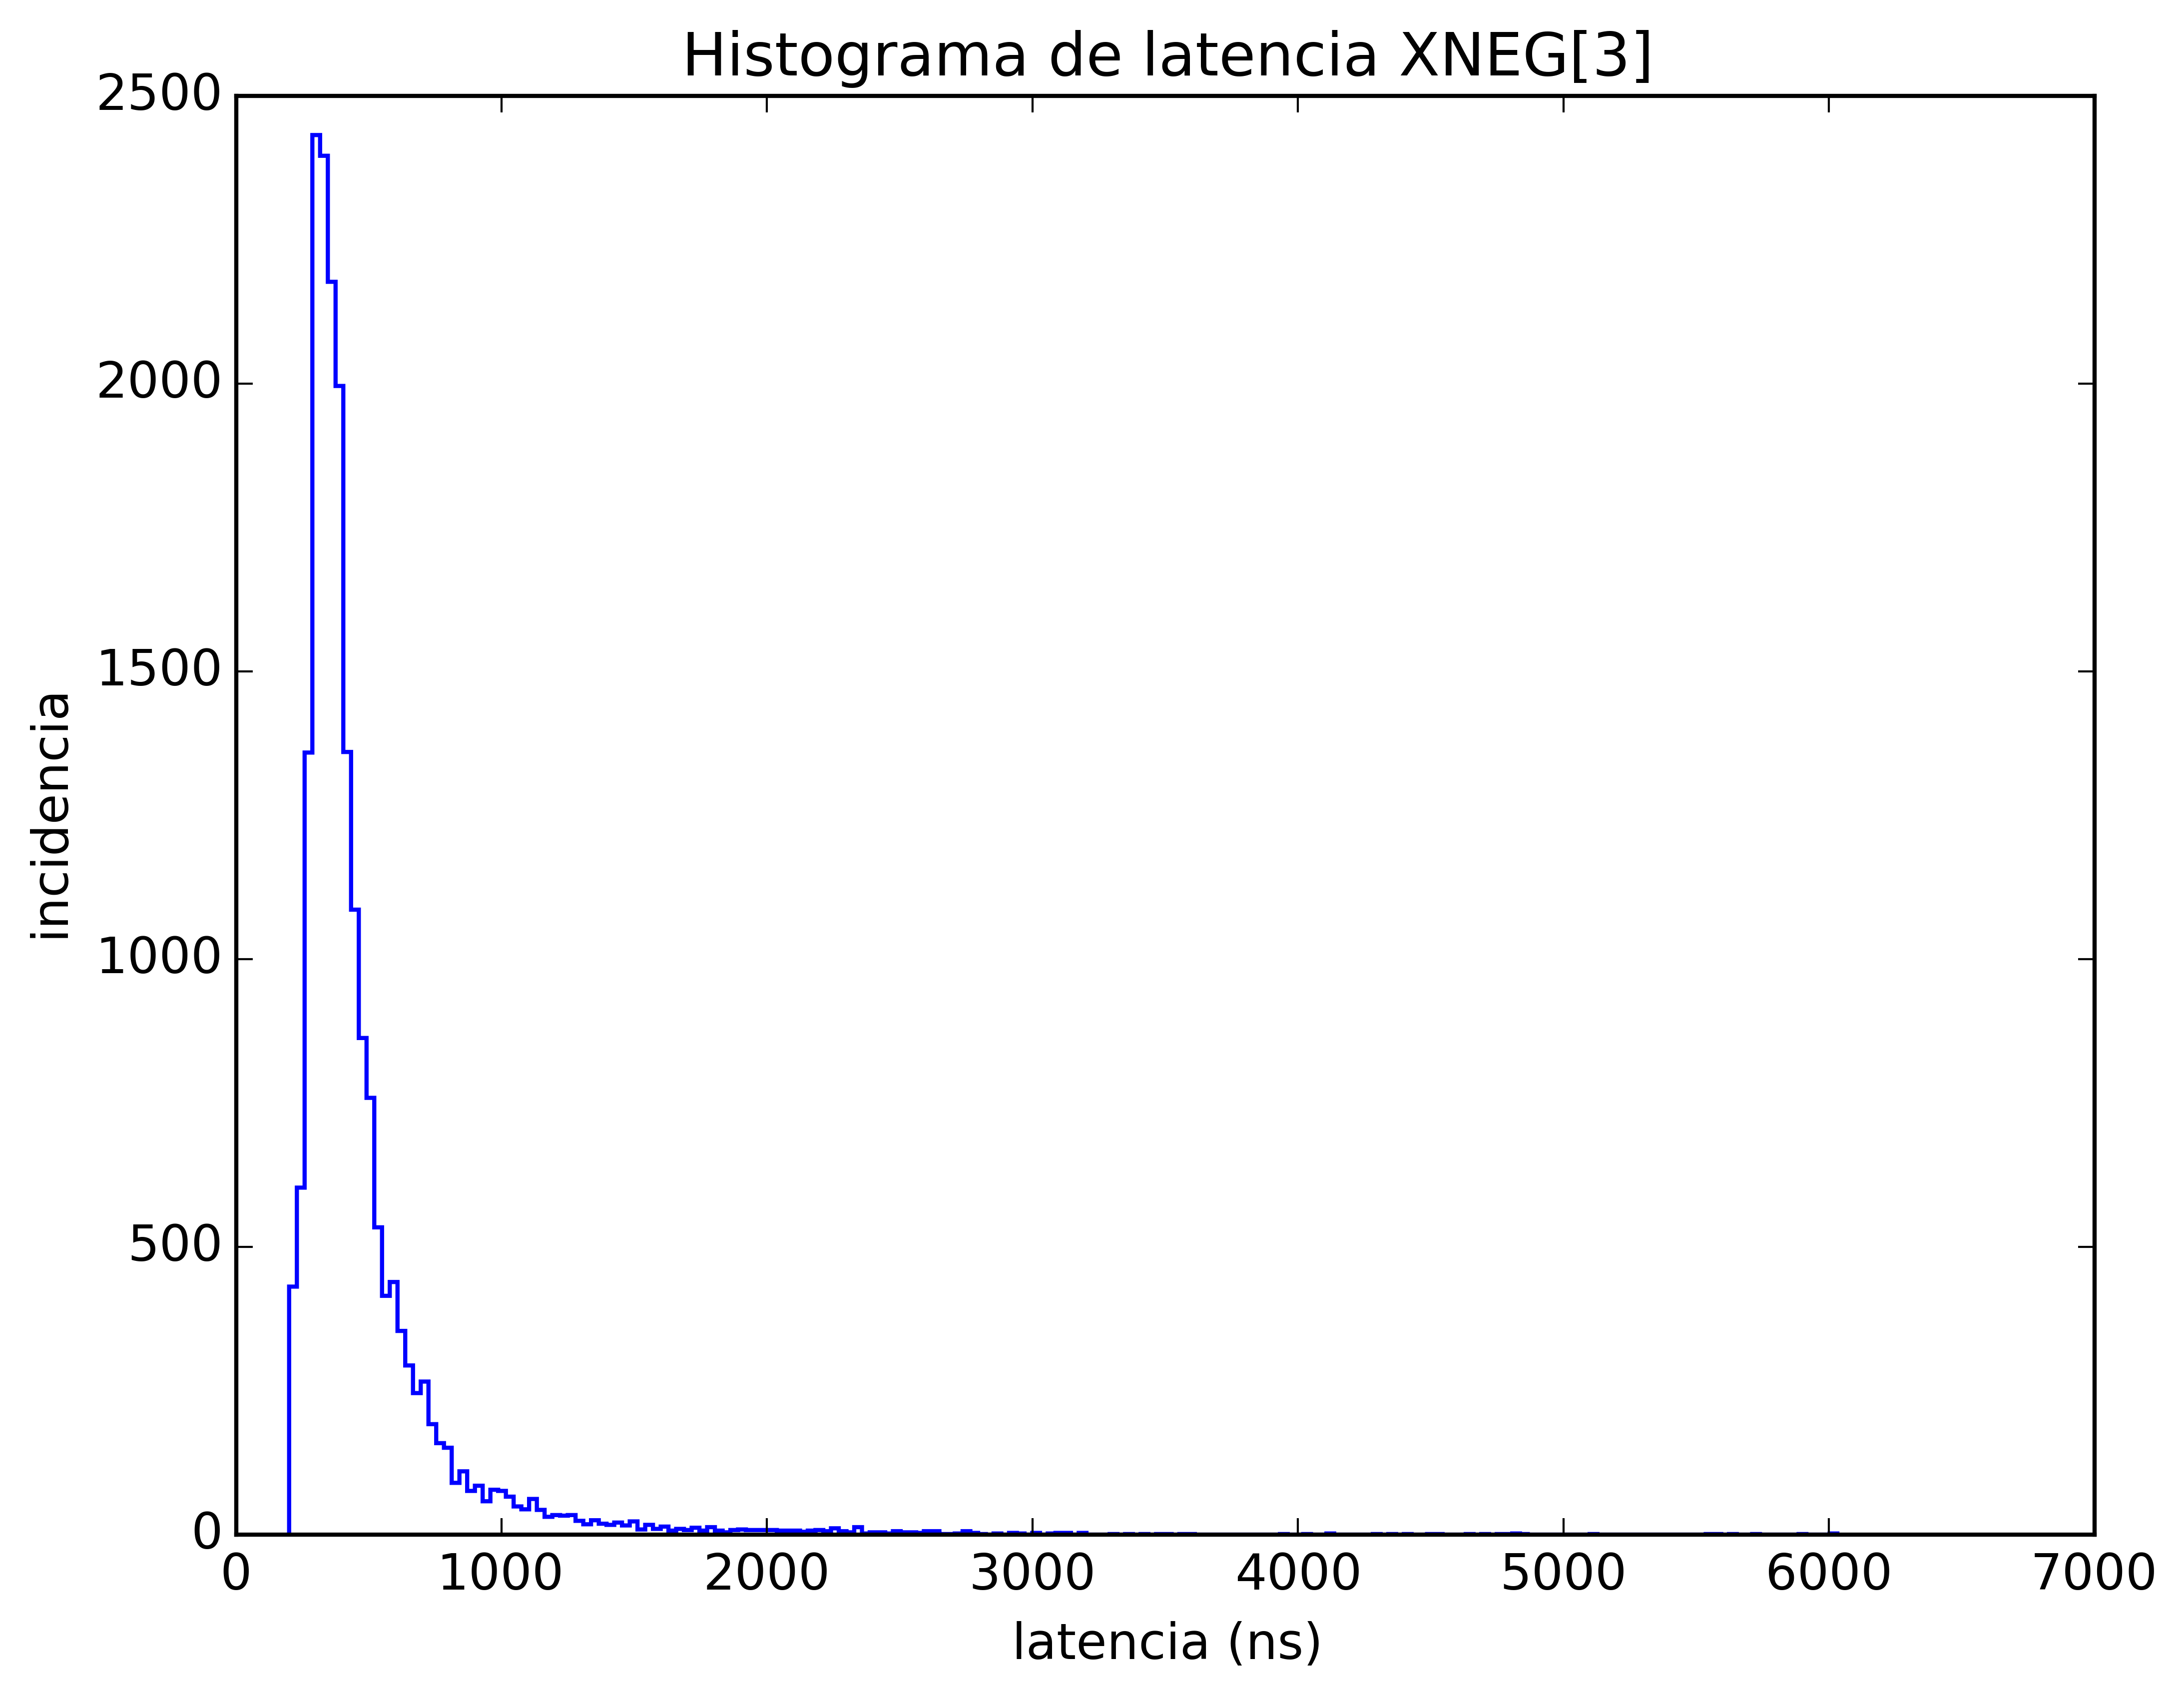
\includegraphics[width=\textwidth]{figures/ch6_histograma_source_3.png}
		    \caption{}
		    \label{fig:histograma_3}
	    \end{subfigure}
	    ~ %add desired spacing between images, e. g. ~, \quad, \qquad, \hfill etc. 
	    %(or a blank line to force the subfigure onto a new line)
	    \begin{subfigure}[b]{0.4\textwidth}
	    	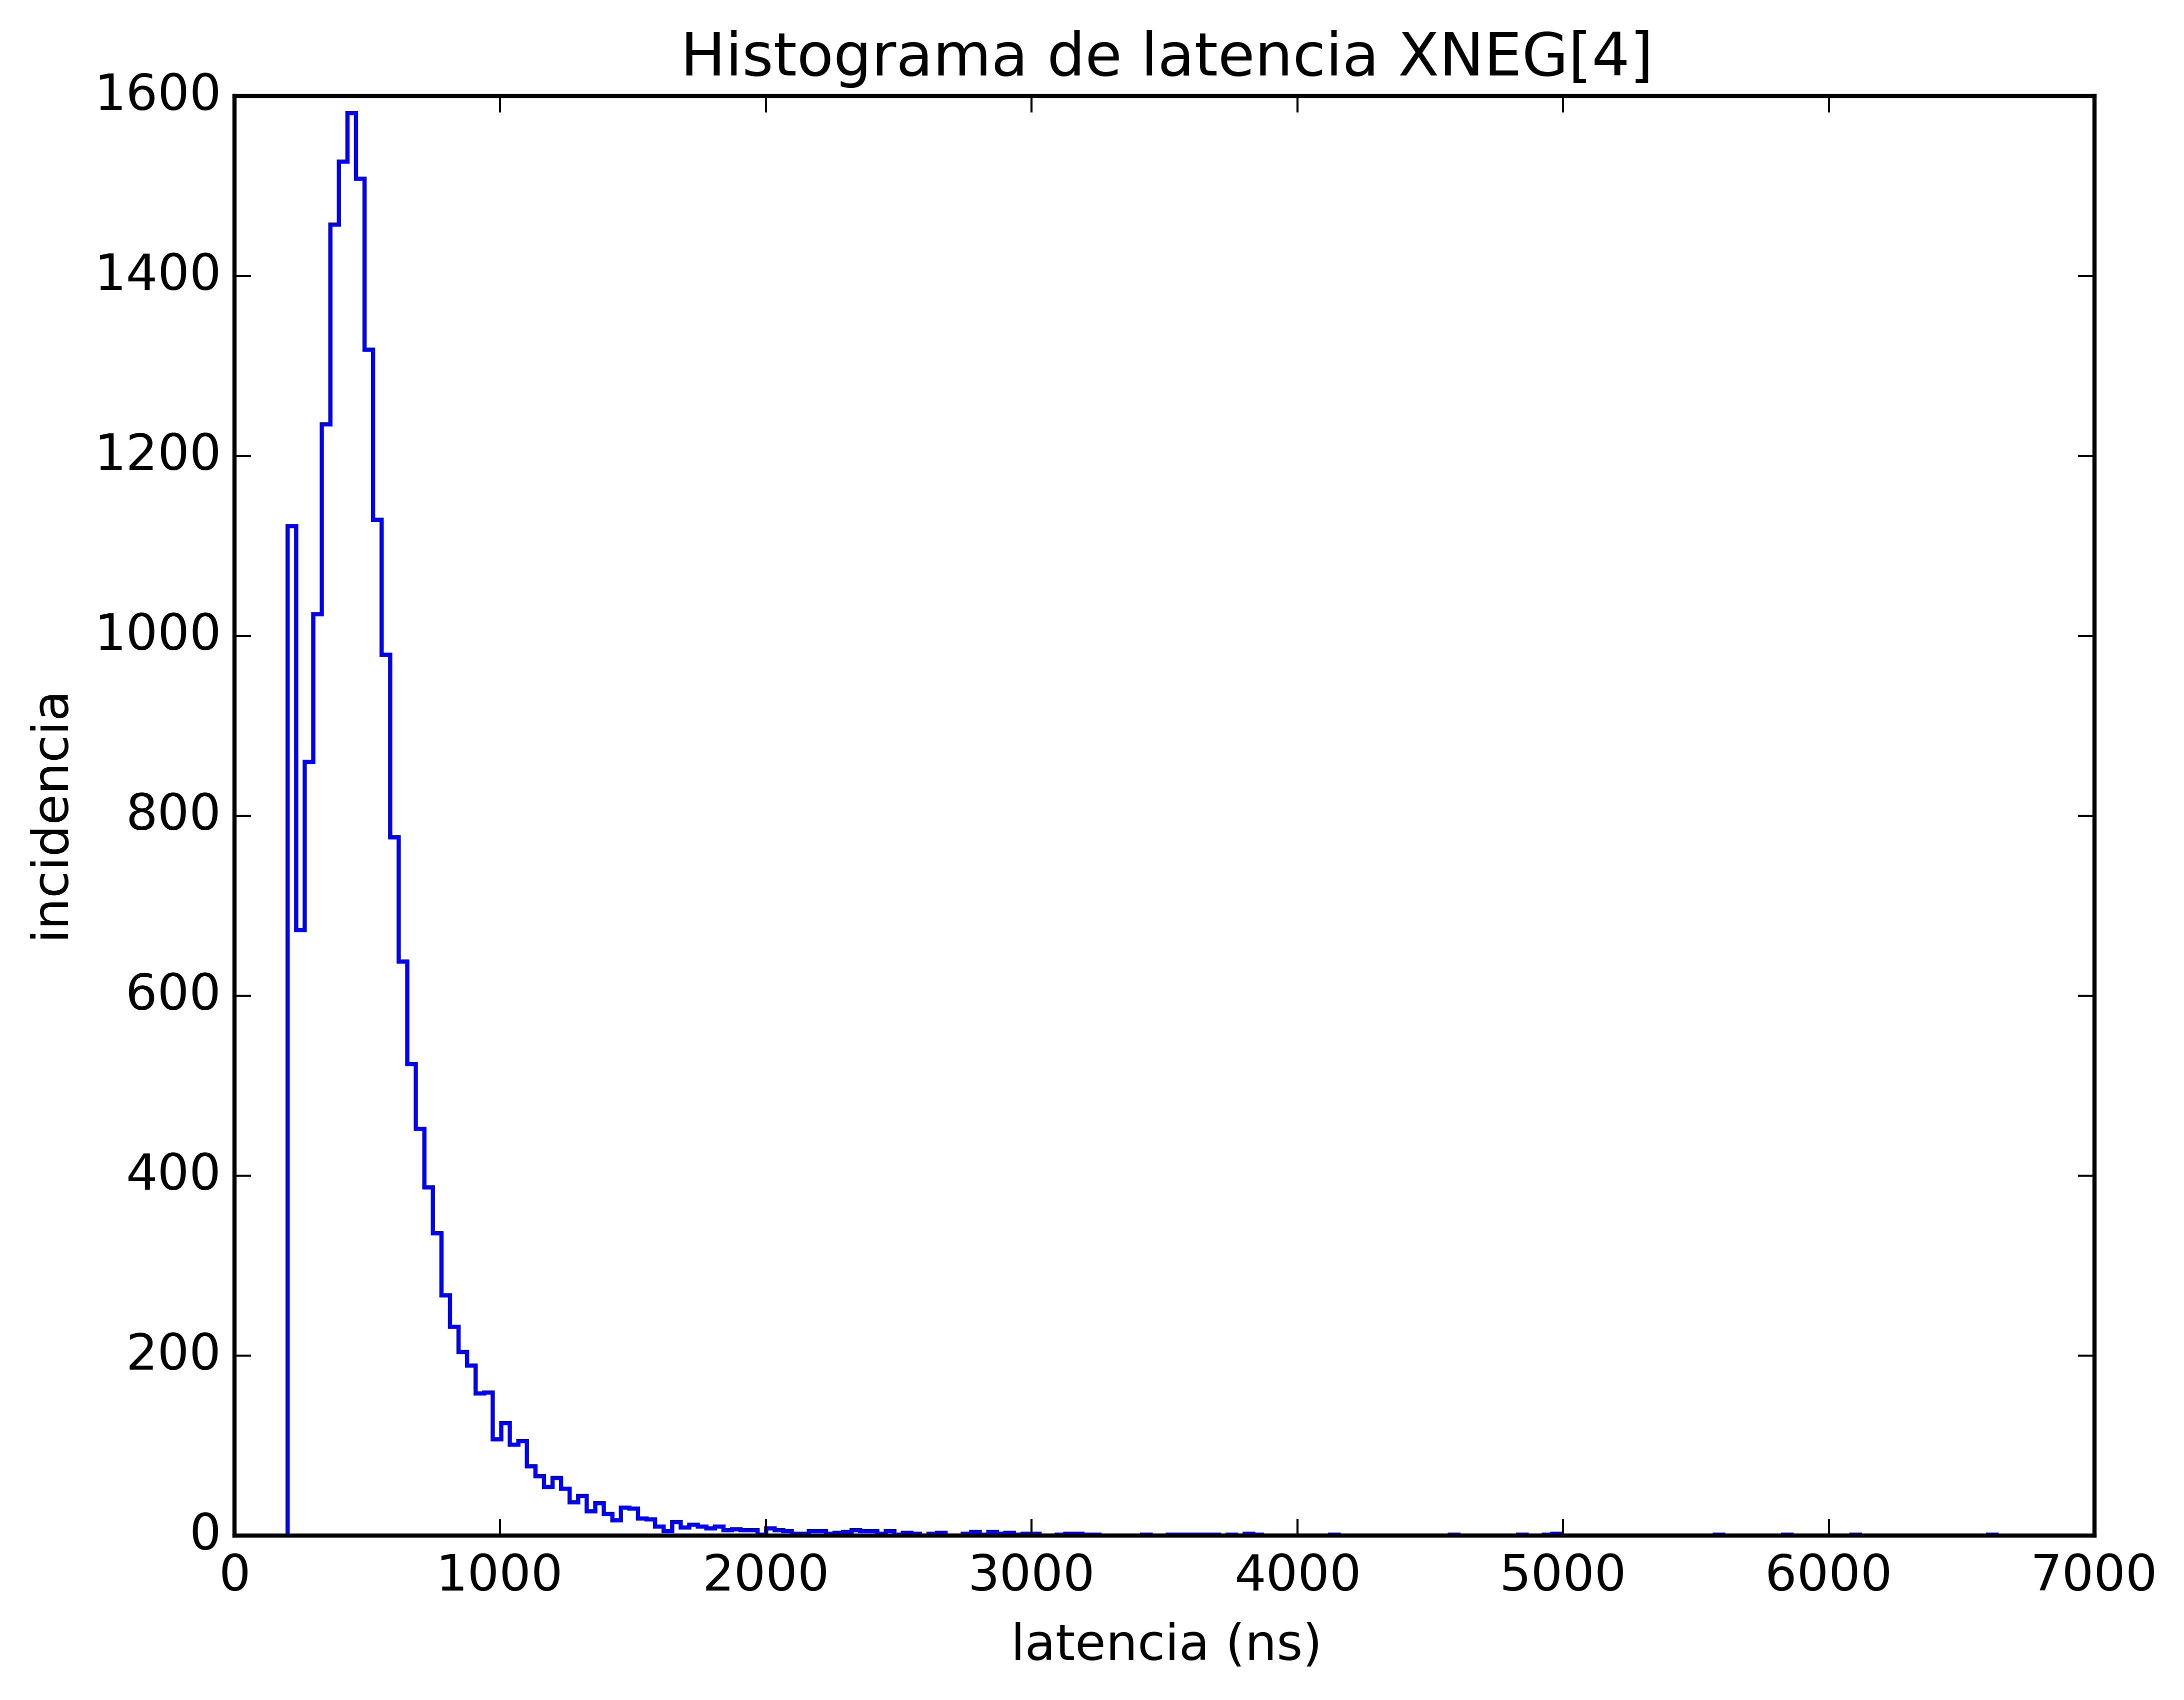
\includegraphics[width=\textwidth]{figures/ch6_histograma_source_4.png}
		    \caption{}
		    \label{fig:histograma_4}
	    \end{subfigure}
	    ~ %add desired spacing between images, e. g. ~, \quad, \qquad, \hfill etc. 
	    %(or a blank line to force the subfigure onto a new line)
	    \begin{subfigure}[b]{0.4\textwidth}
	    	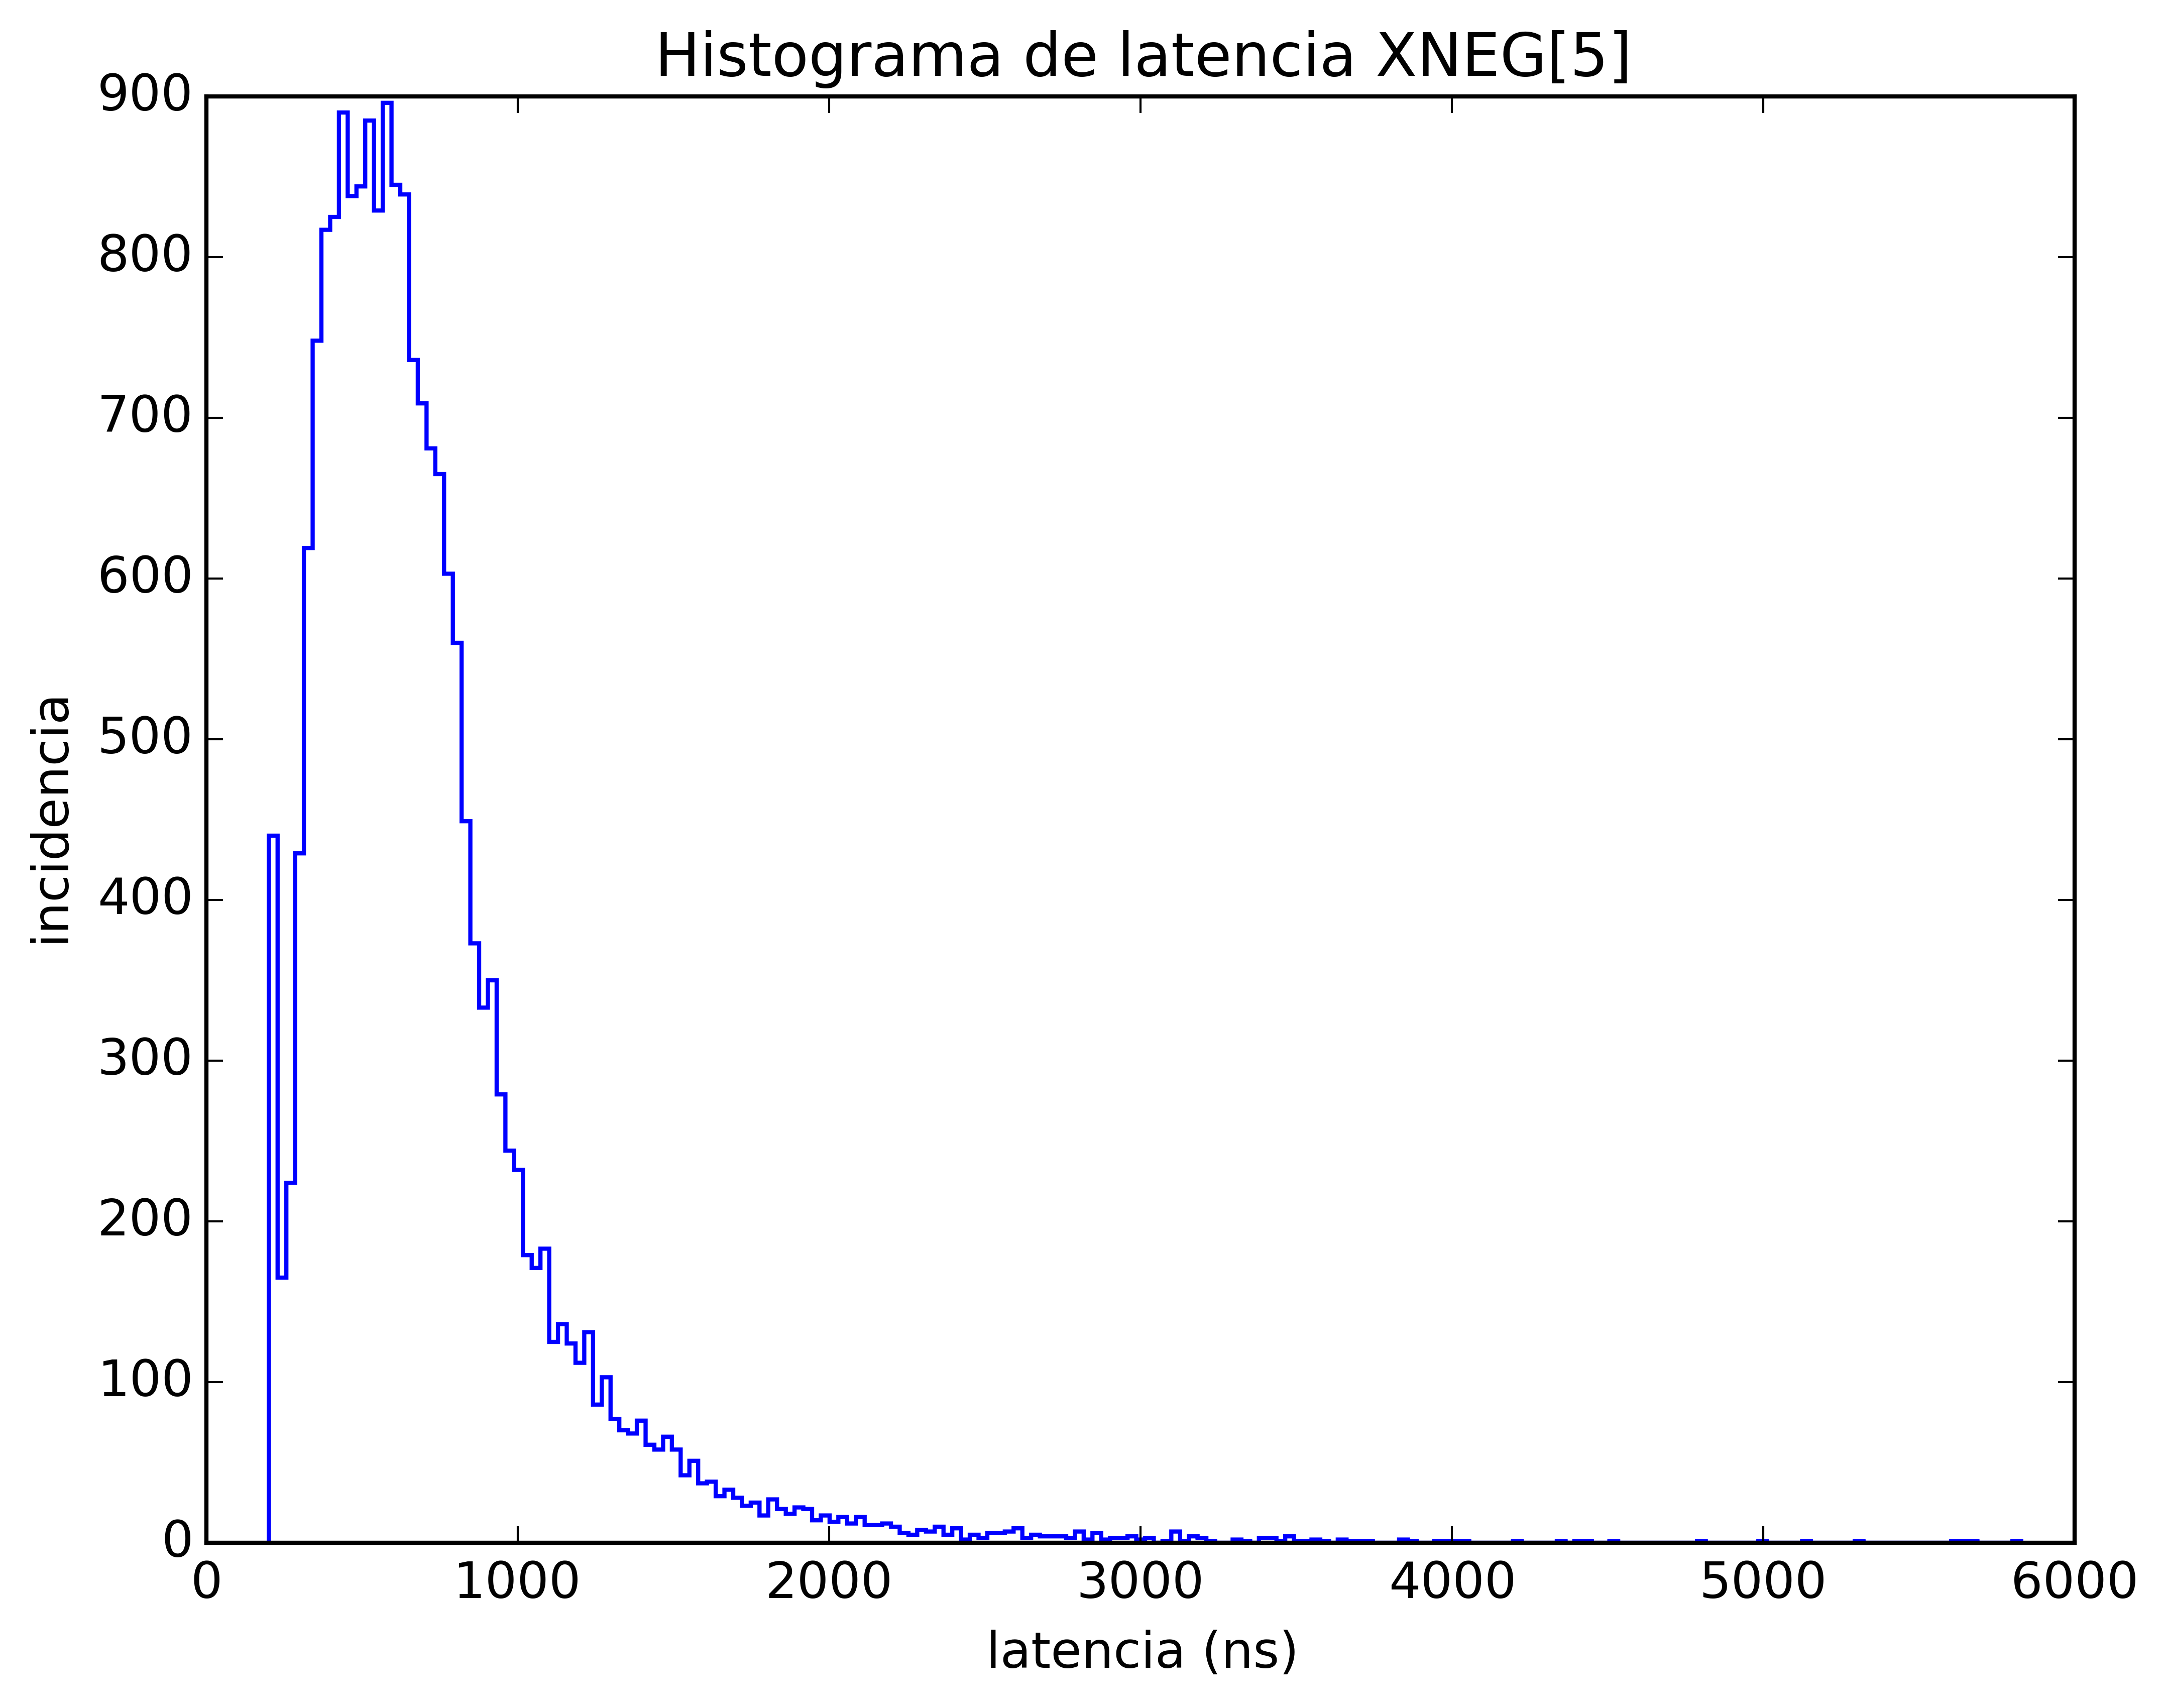
\includegraphics[width=\textwidth]{figures/ch6_histograma_source_5.png}
		    \caption{}
		    \label{fig:histograma_5}
	    \end{subfigure}
	   %
    \end{center}
    \caption{%
        Histogramas de latencia de recepción de paquetes para puertos en dirección \textit{x-}.
     }%
   \label{fig:ch6_histogramas_1}
\end{figure}

\begin{figure}[ht!]
\captionsetup[subfigure]{justification=centering}
     \begin{center}
%
        \begin{subfigure}[b]{0.4\textwidth}
        	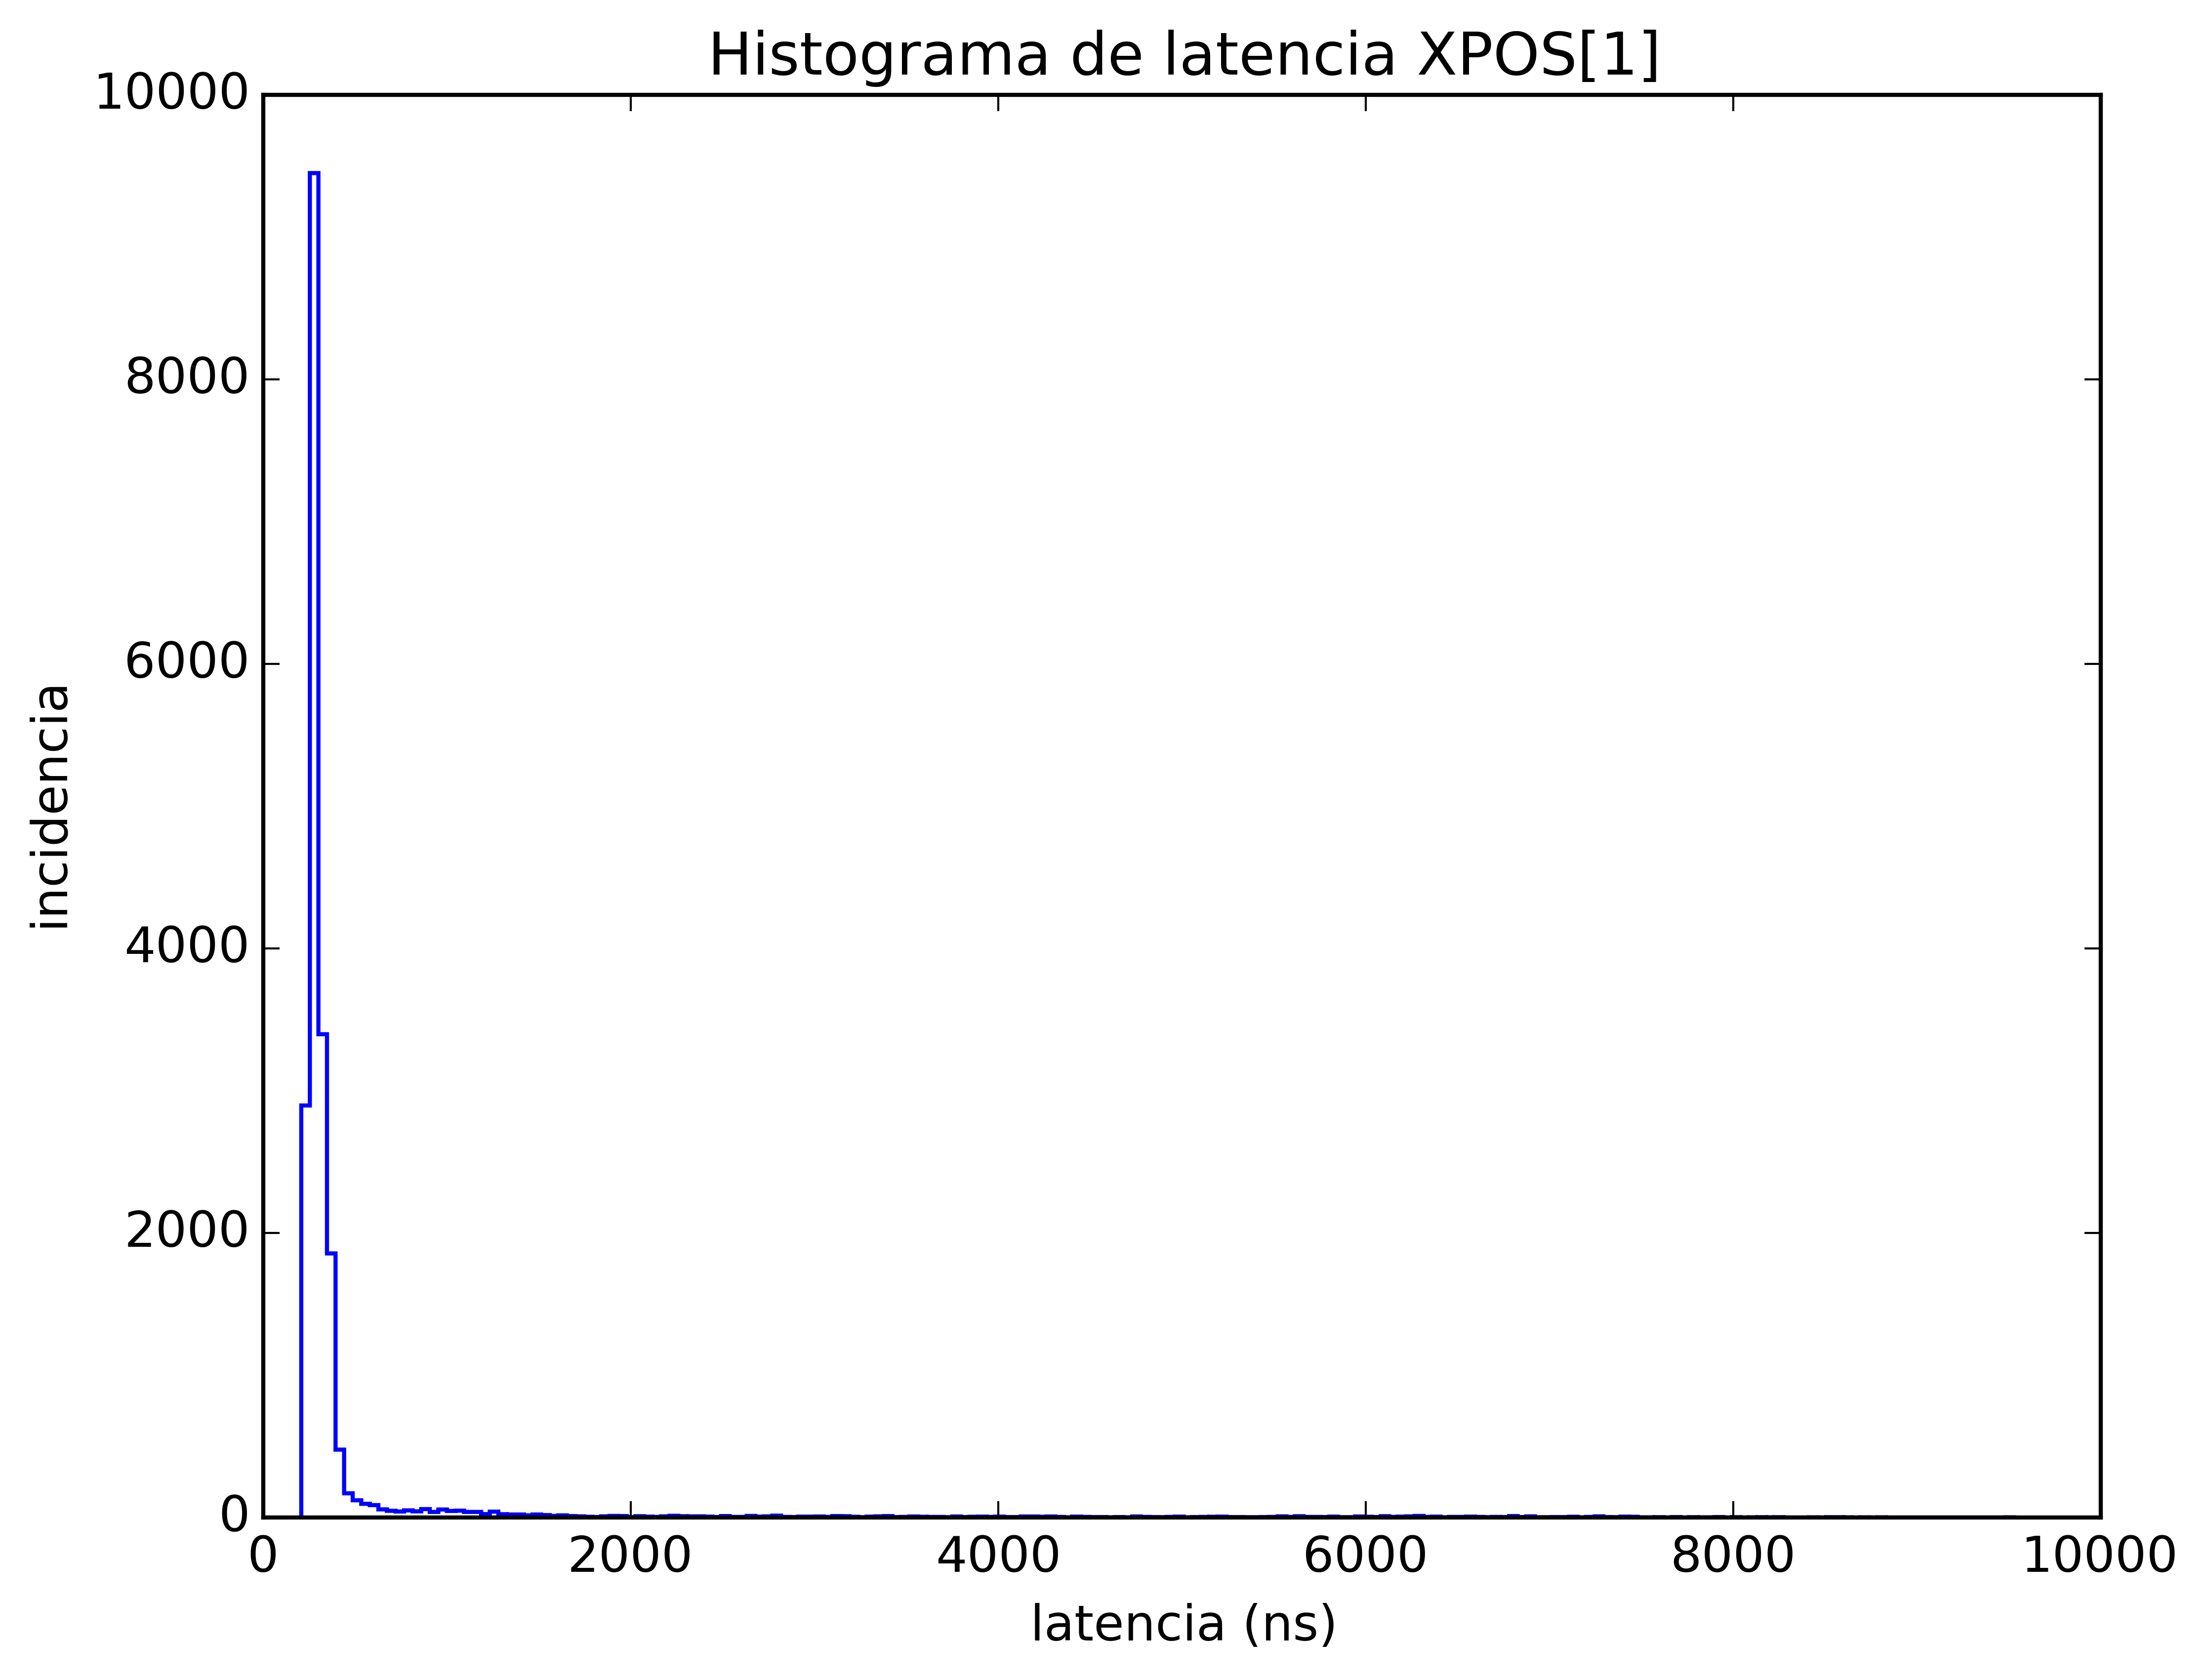
\includegraphics[width=\textwidth]{figures/ch6_histograma_source_6.png}
		    \caption{}
		    \label{fig:histograma_6}
	    \end{subfigure}
	    ~ %add desired spacing between images, e. g. ~, \quad, \qquad, \hfill etc. 
	      %(or a blank line to force the subfigure onto a new line)
	    \begin{subfigure}[b]{0.4\textwidth}
	    	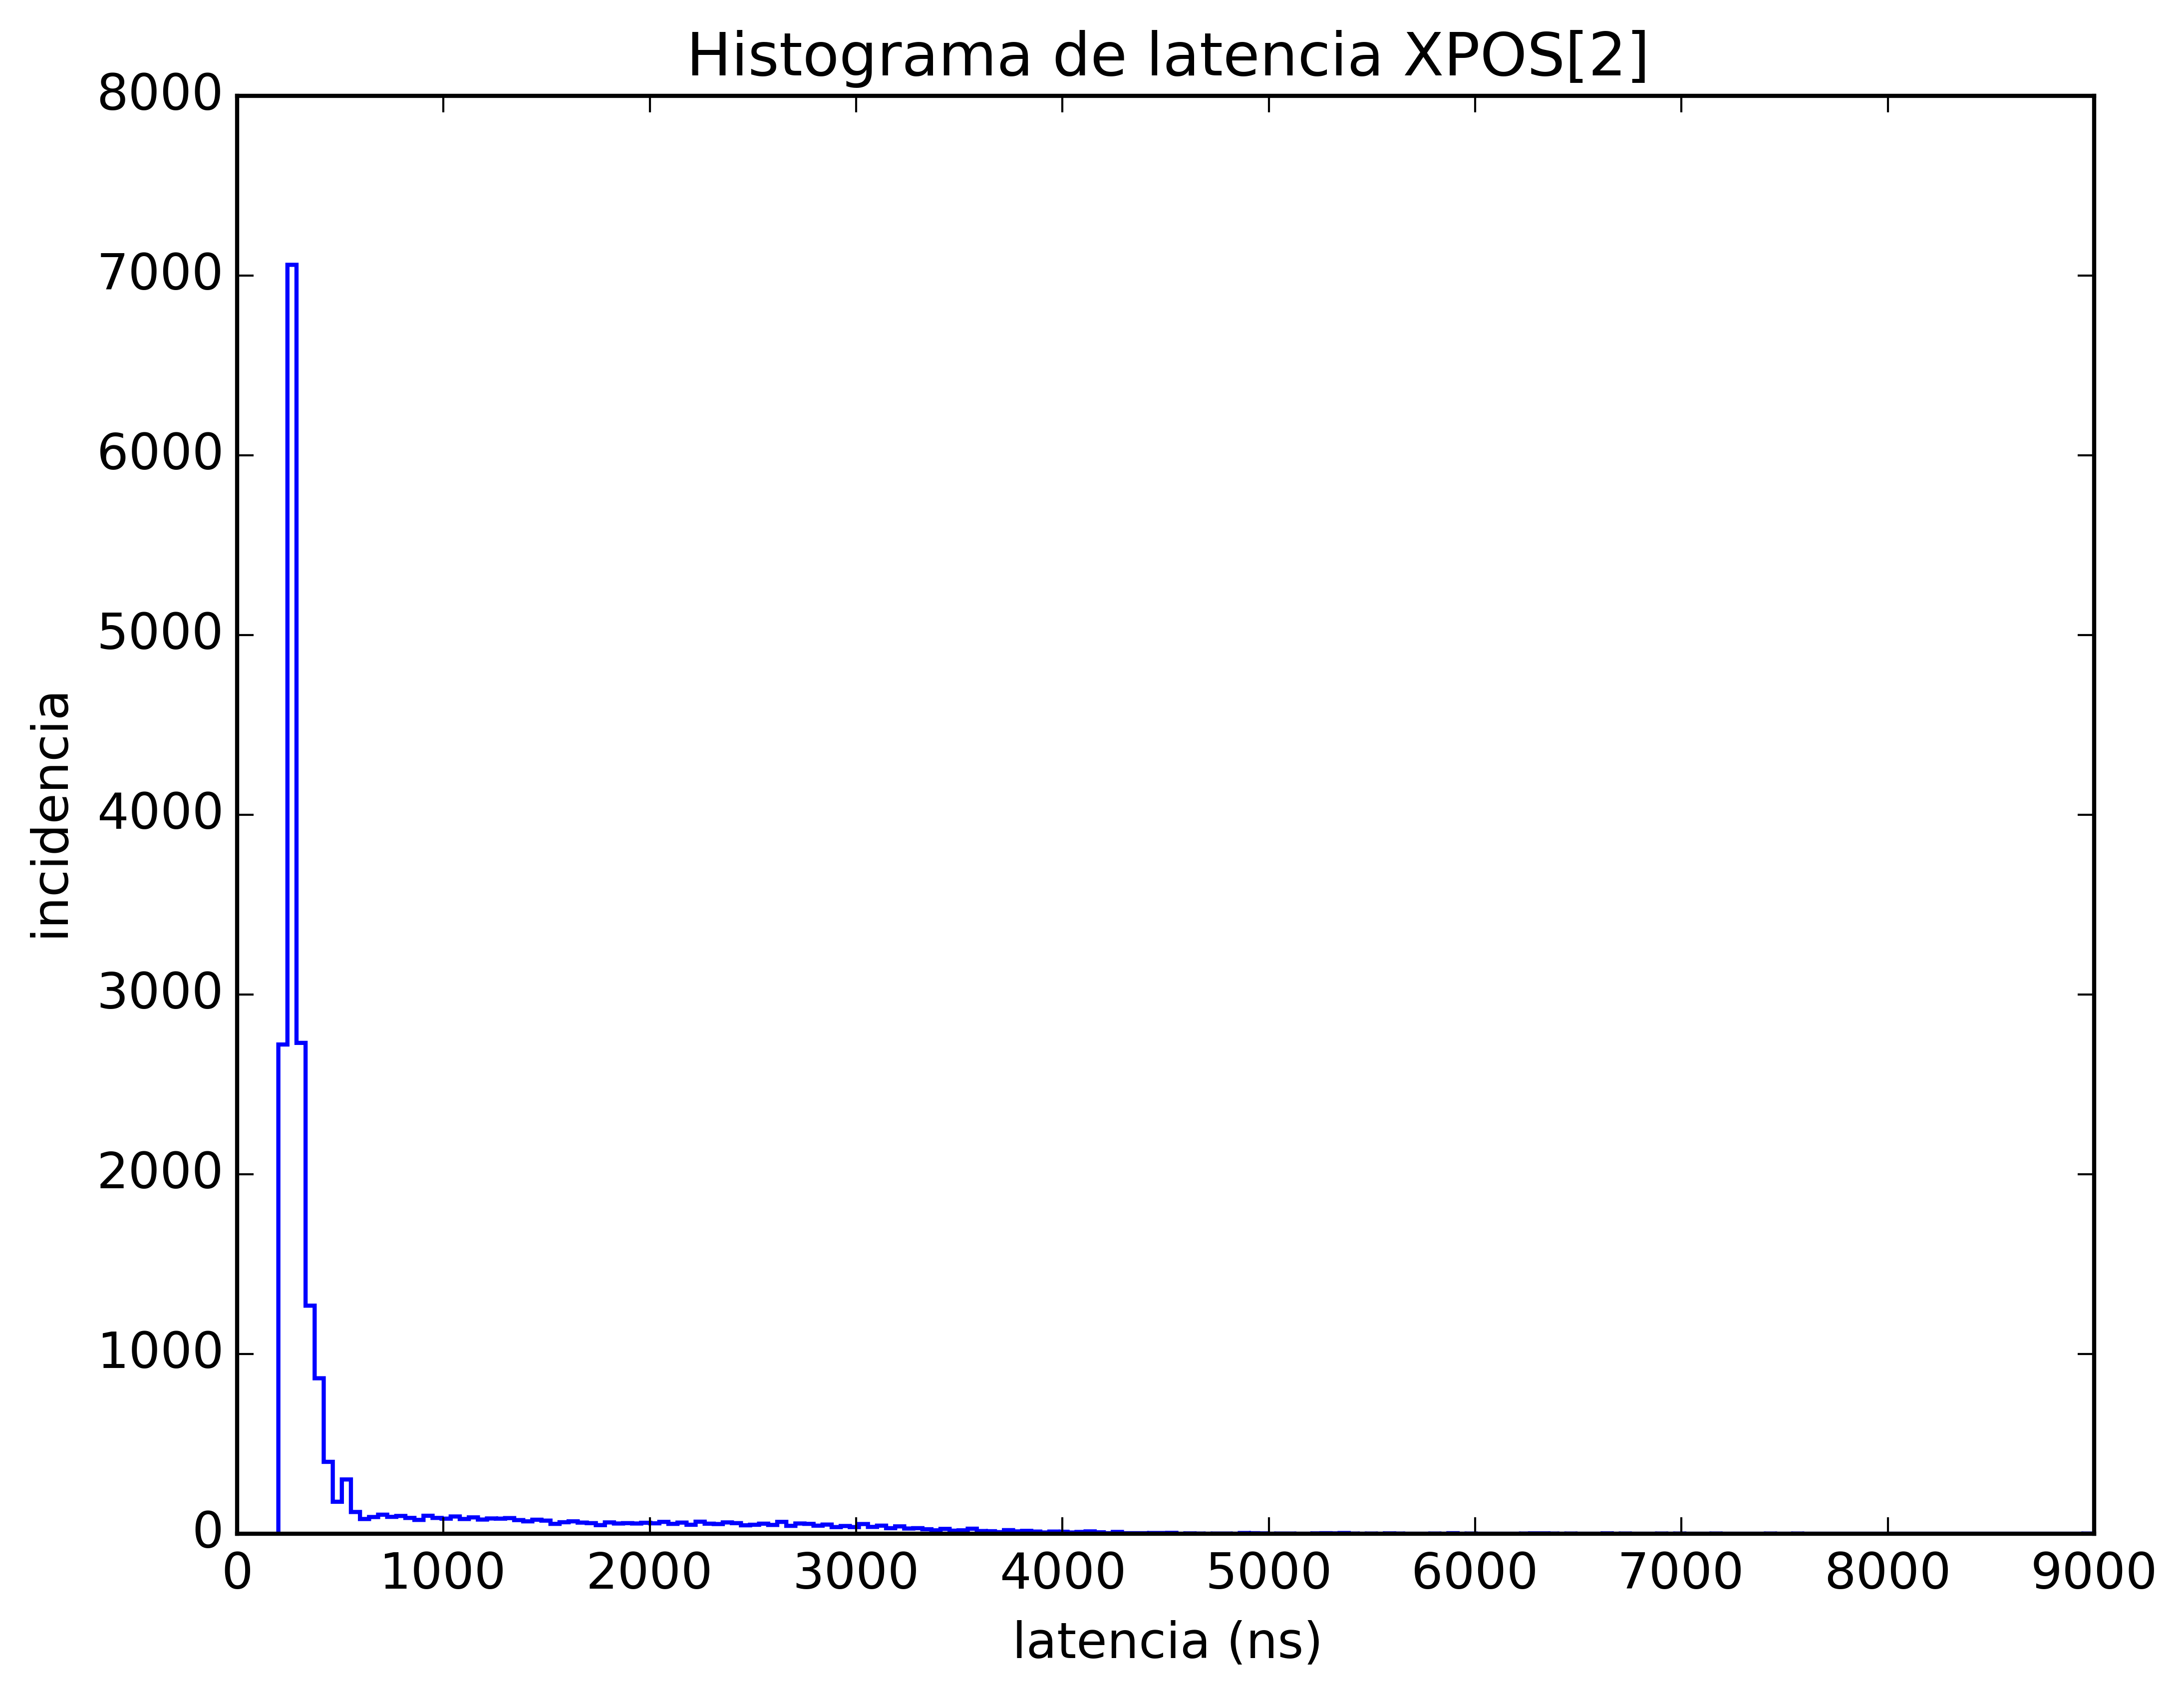
\includegraphics[width=\textwidth]{figures/ch6_histograma_source_7.png}
		    \caption{}
		    \label{fig:histograma_7}
	    \end{subfigure}
	    ~ %add desired spacing between images, e. g. ~, \quad, \qquad, \hfill etc. 
	    %(or a blank line to force the subfigure onto a new line)
	    \begin{subfigure}[b]{0.4\textwidth}
	    	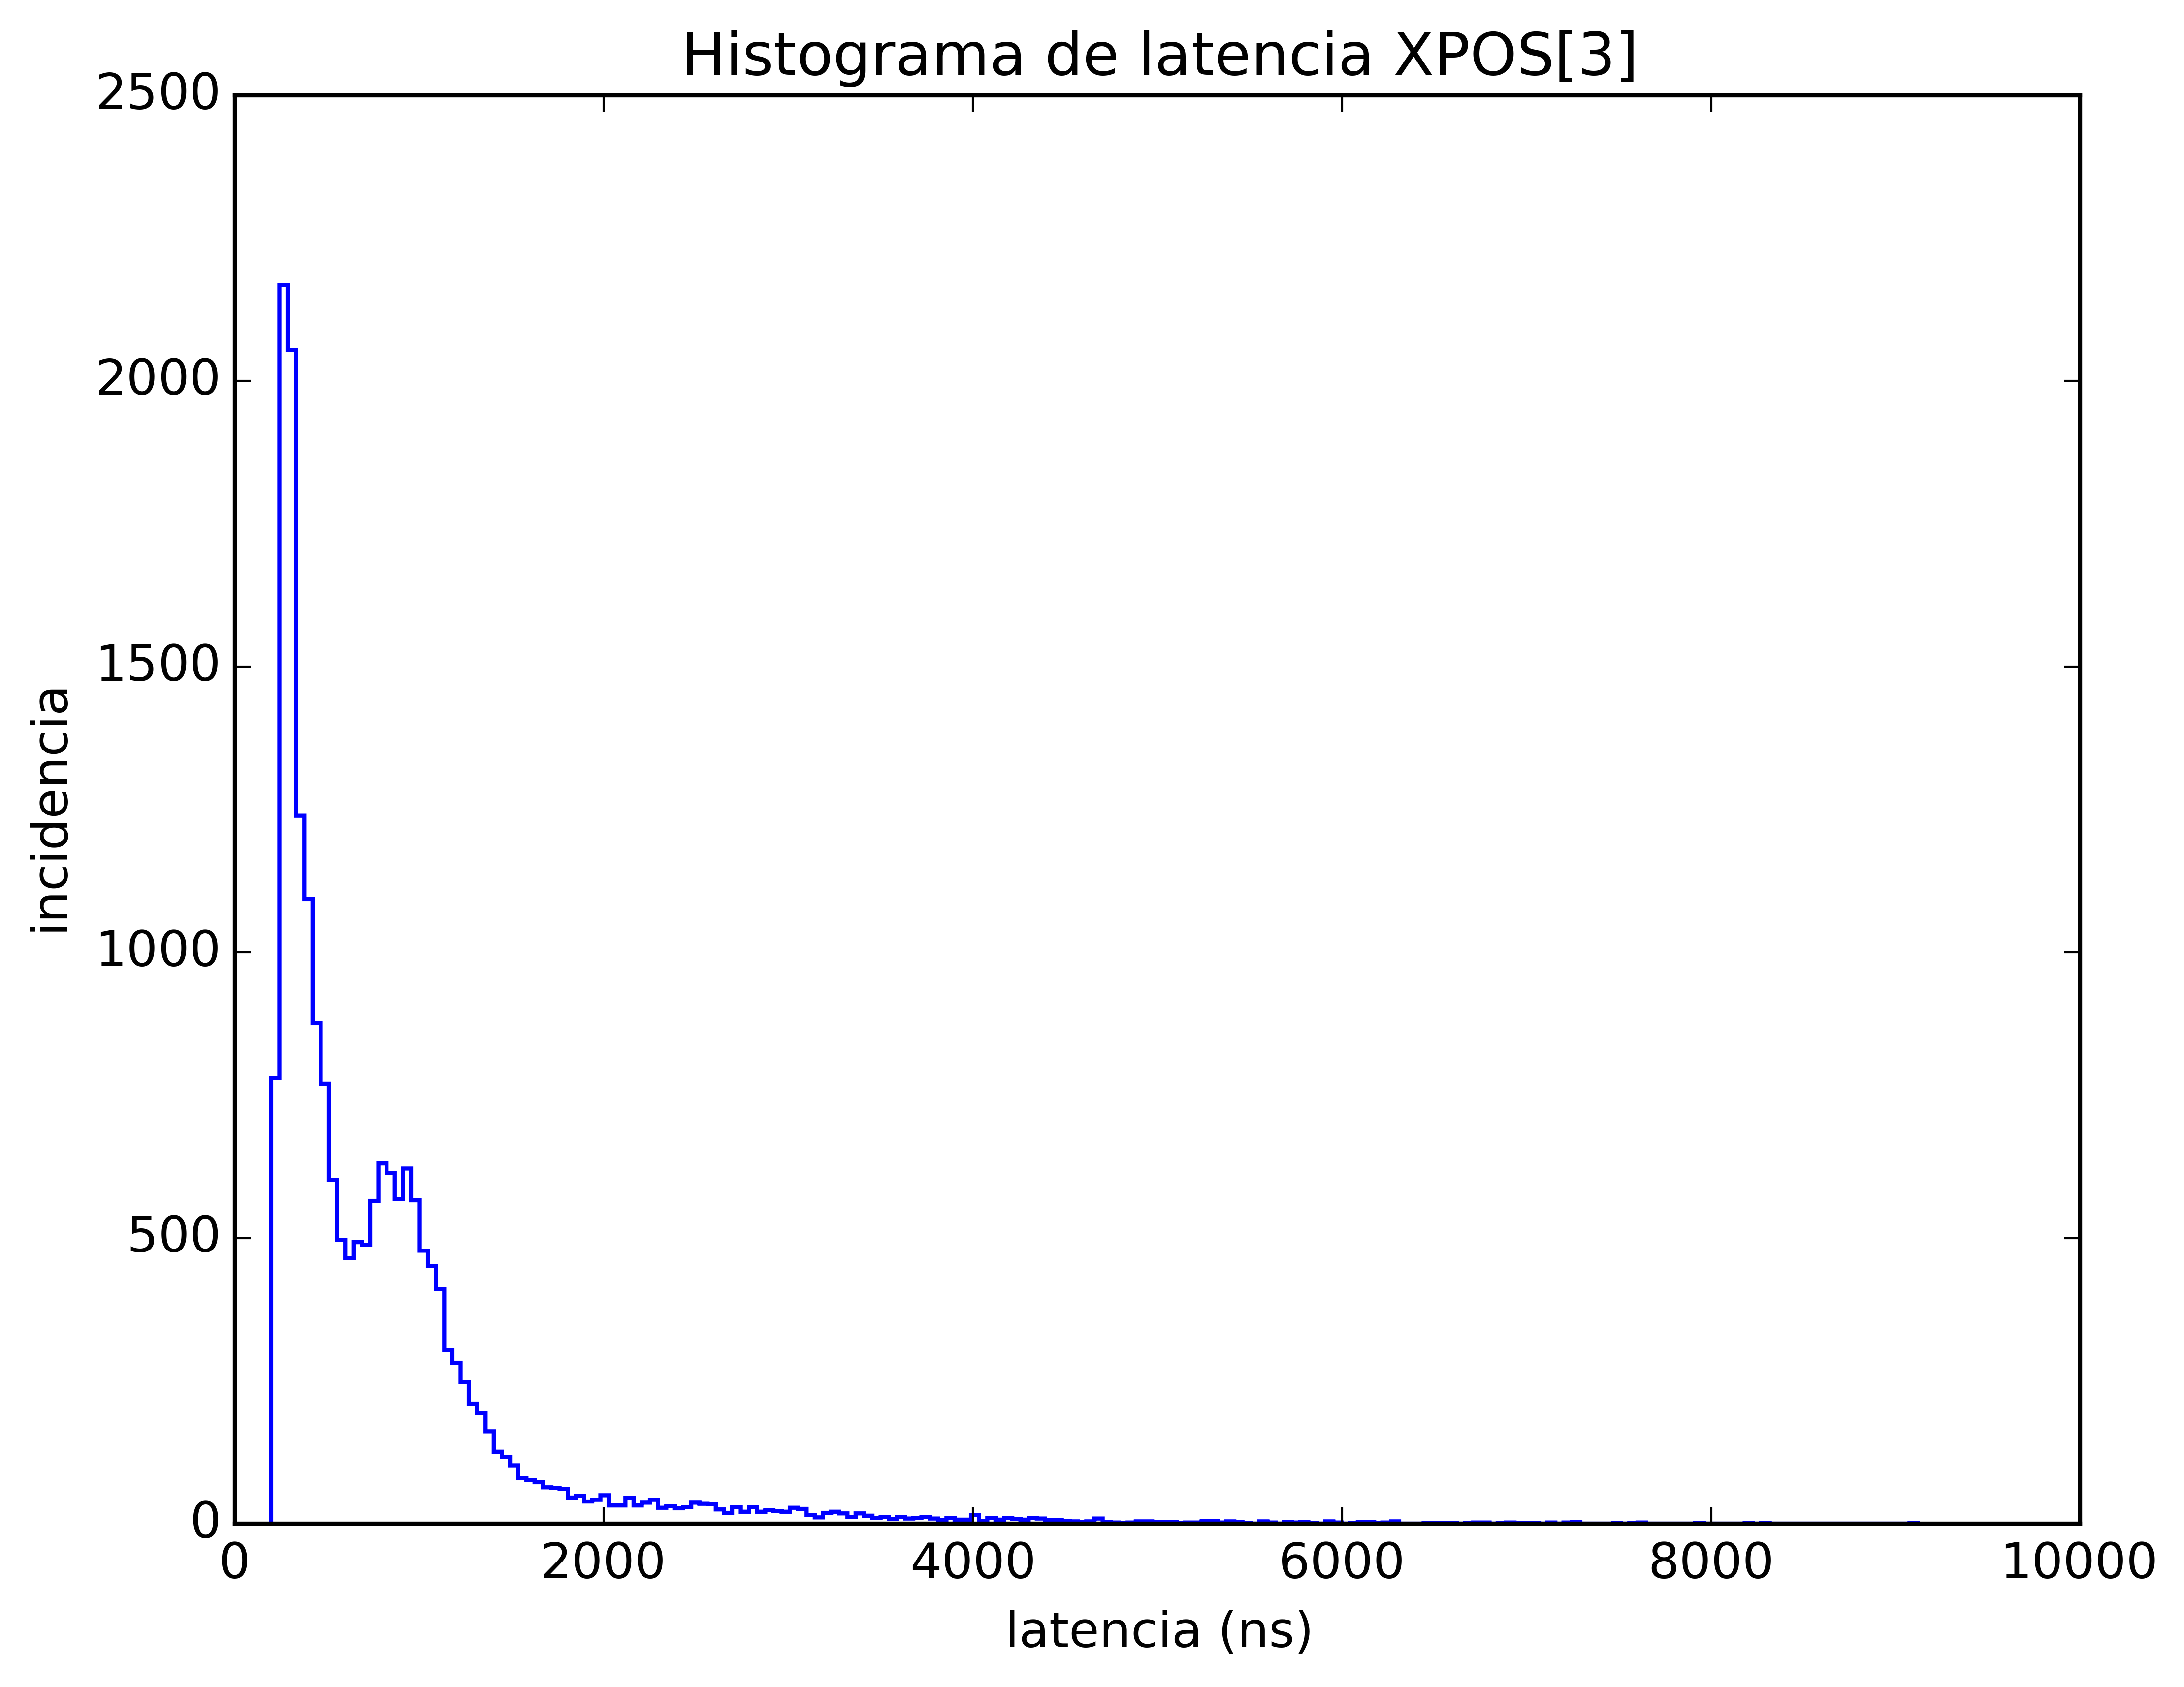
\includegraphics[width=\textwidth]{figures/ch6_histograma_source_8.png}
		    \caption{}
		    \label{fig:histograma_8}
	    \end{subfigure}
	    ~ %add desired spacing between images, e. g. ~, \quad, \qquad, \hfill etc. 
	    %(or a blank line to force the subfigure onto a new line)
	    \begin{subfigure}[b]{0.4\textwidth}
	    	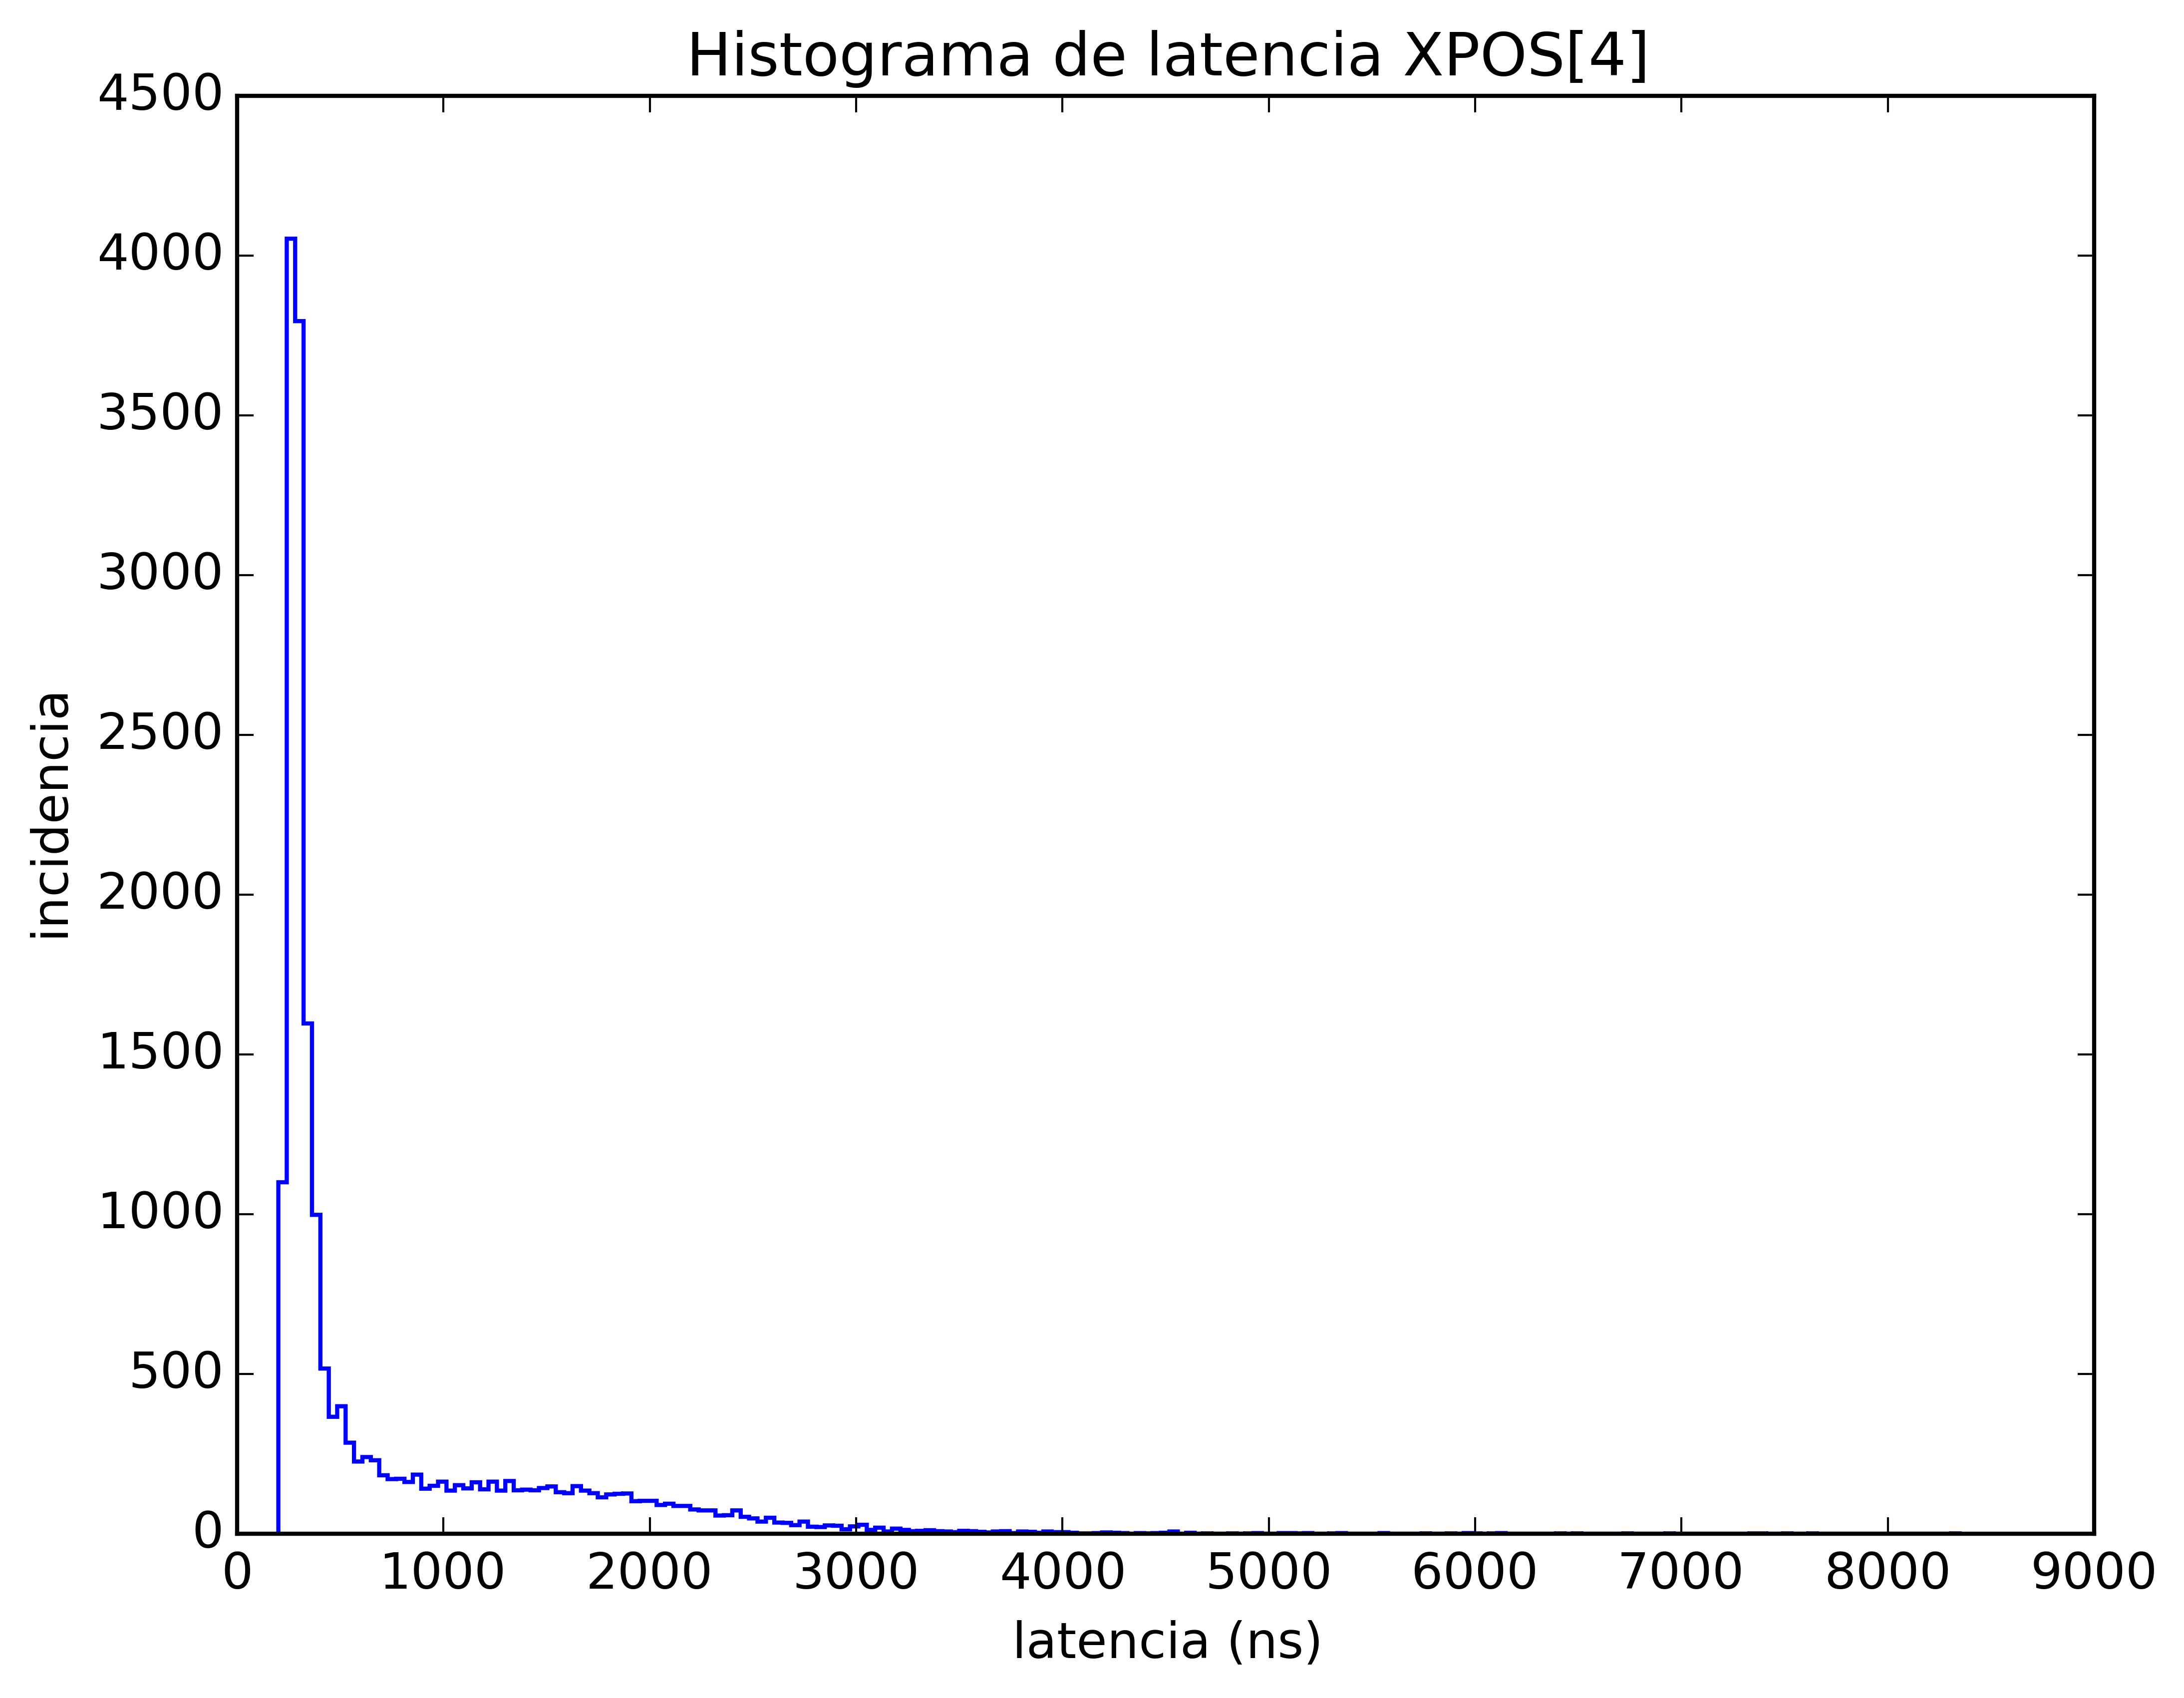
\includegraphics[width=\textwidth]{figures/ch6_histograma_source_9.png}
		    \caption{}
		    \label{fig:histograma_9}
	    \end{subfigure}
	    ~ %add desired spacing between images, e. g. ~, \quad, \qquad, \hfill etc. 
	    %(or a blank line to force the subfigure onto a new line)
	    \begin{subfigure}[b]{0.4\textwidth}
	    	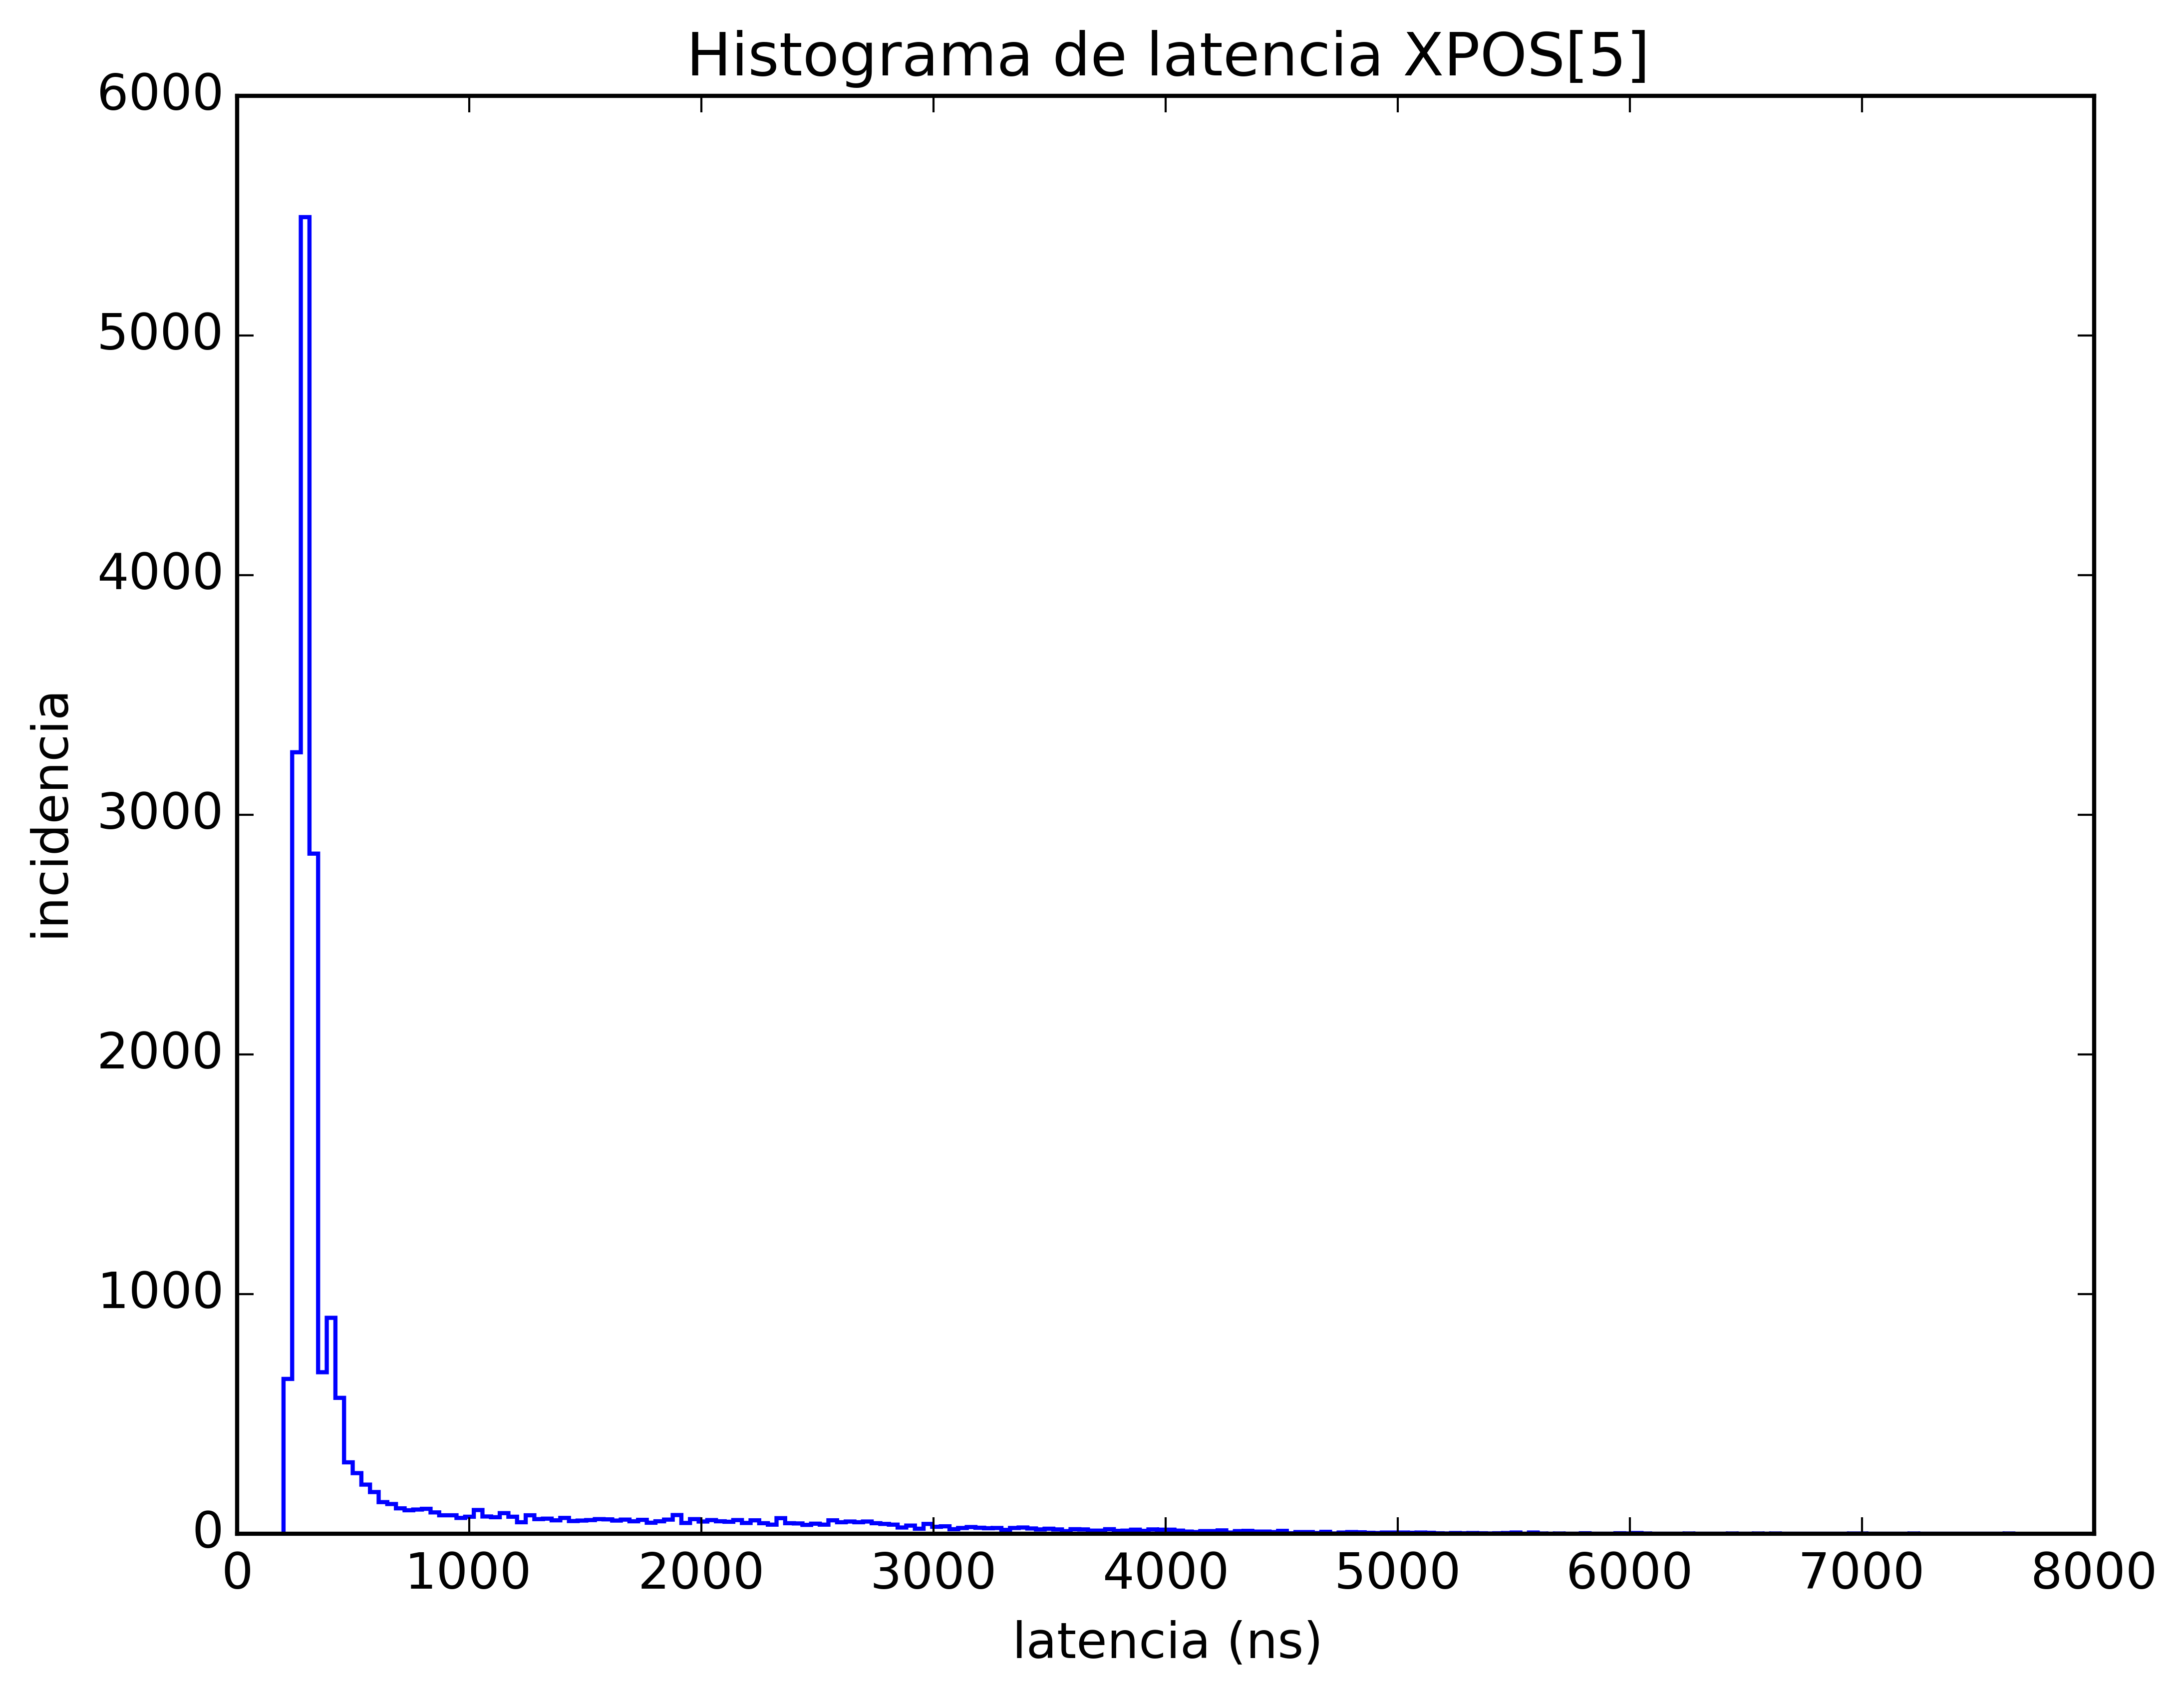
\includegraphics[width=\textwidth]{figures/ch6_histograma_source_10.png}
		    \caption{}
		    \label{fig:histograma_10}
	    \end{subfigure}
	   %
    \end{center}
    \caption{%
        Histogramas de latencia de recepción de paquetes para puertos en dirección \textit{x+}.
     }%
   \label{fig:ch6_histogramas_2}
\end{figure}